\documentclass[]{article}

\usepackage{natbib}
\bibliographystyle{style/amnatnat}

\usepackage{amsmath,amssymb,bm}

\usepackage[colorlinks=true, citecolor=blue, urlcolor=blue, linkcolor = blue]{hyperref}

\usepackage{graphicx}
\usepackage{grffile}
\graphicspath{{../figures/}}
\usepackage{epstopdf}
\epstopdfsetup{outdir=./}

\usepackage{tikz}
\usetikzlibrary{positioning}
\usetikzlibrary{calc}
\usepackage{pgfmath,pgffor}
\usepackage{ifthen}

\usepackage{color}
\definecolor{darkblue}{rgb}{0.2472, 0.24, 0.6}
\definecolor{darkred}{rgb}{0.6, 0.24, 0.442893}
\newcommand{\gc}[1]{\textcolor{orange}{#1}}
\newcommand{\mo}[1]{\textcolor{red}{#1}}

\usepackage{fullpage}
\usepackage{lineno}
\usepackage{setspace}

\usepackage{authblk}
\makeatletter
\let\@fnsymbol\@arabic
\makeatother

%%%%%%%%%%%%%%%%%%%%%%%%%%%%%%%%%%%%%%%%%%%%%%%%%%%%
\title{Genetic signatures of evolutionary rescue by a selective sweep}
\author[*]{Matthew M.\ Osmond\thanks{mmosmond@ucdavis.edu}}
\author[*]{Graham Coop}
\affil[*]{Center for Population Biology and Department of Evolution and Ecology, University of California, Davis, California 95616}
\date{}
\renewcommand\Affilfont{\itshape\small}

%%%%%%%%%%%%%%%%%%%%%%%%%%%%%%%%%%%%%%%%%%%%%%%%%%%%
\begin{document}
%\doublespacing

%%%%%%%%%%%%%%%%%%%%%%%%%%%%%%%%%%%%%%%%%%%%%%%%%%%
\maketitle

%\linenumbers
%%%%%%%%%%%%%%%%%%%%%%%%%%%%%%%%%%%%%%%%%%%%%%%%%%%
\section*{Abstract}
\label{sec:abstract}

One of the most useful models in population genetics is that of a selective sweep and the consequent hitch-hiking of linked neutral alleles.
While variations on this model typically assume constant population size, many instances of strong selection and rapid adaptation in nature may co-occur with complex demography.
Here we extend the hitch-hiking model to evolutionary rescue, where adaptation and demography not only co-occur but are intimately entwined. 
Our results show how this feedback between demography and evolution determines the genetic signatures of evolutionary rescue, and how these differ from the signatures of sweeps in populations of constant size.
In particular, we find rescue to harden sweeps from standing variance or new mutation (but not from migration), reduce nucleotide diversity both at the selected site and genome-wide, and increase the range of observed Tajima's $D$ values.
For a given rate of population decline, the feedback between demography and evolution makes all of these differences more dramatic under weaker selection, where bottlenecks are prolonged. 
It is likely difficult to infer the co-incident timing of the sweep and bottleneck from these simple signatures, nevermind a feedback between them. 
However, temporal samples spanning contemporary rescue events may offer one way forward.

%%%%%%%%%%%%%%%%%%%%%%%%%%%%%%%%%%%%%%%%%%%%%%%%%%%
\section*{Introduction}
\label{sec:intro}

The simple models used to predict the genetic signatures of selective sweeps have been incredibly helpful in understanding and identifying population genetic signals of adaptation (e.g., \citealp{smith1974hitch,kaplan1989hitchhiking}; reviewed in \citealp{stephan2019selective}). 
These models are usually based on constant-sized, Wright-Fisher populations.
Meanwhile, many instances of adaptation -- and thus selective sweeps -- in nature will co-occur with complex demography.
In fact, many of the most well-known examples of selective sweeps have arisen following a rather extreme and sudden change in the environment (e.g., after the application of insecticides, \citealp{sedghifar2016genomic}, or antimalarial drugs, \citealp{nair2003selective}), which could have simultaneously imposed sharp demographic declines.
Attempts to capture such complex demographic scenarios typically impose qualitatively appropriate changes in population size \citep[e.g.,][]{hermisson2005soft}.
Indeed, a number of studies have explored the genetic signatures of selective sweeps during demographic bottlenecks \citep[e.g.,][]{innan2004pattern,teshima2006reliable,wilson2014soft}.
However, these demographies are nearly always chosen in the absence of an explicit population model and independently of evolution.

Here we model selective sweeps in a scenario where demography and adaptive evolution are not independent.
In particular we model an instance of evolutionary rescue (\citealp{gomulkiewicz1995does}; reviewed in \citealp{bell2017evolutionary}), where a sudden environmental change causes population decline that is reverted by a selective sweep.
Under this framework, rescue is a simultaneous demographic bottleneck and selective sweep, where each affects the other.
First, because the mean absolute fitness of the population changes with the beneficial allele's frequency, the depth and duration of the bottleneck depends on the dynamics of the selective sweep, i.e., evolution affects demography.
Second, the probability that the beneficial allele establishes depends on the rate of population decline, i.e., demography affects evolution.
Together, this feedback between demography and evolution restricts the range of dynamics that are possible, and therefore also restricts the range of genetic signatures we should expect to observe.
Our goal here is to describe the range of genetic signatures that (this model of) evolutionary rescue allows, to help elucidate how rescue may obscure inferences of past selection and demography and to identify patterns that could be used to infer rescue in nature.

Most theory on evolutionary rescue to date \citep[reviewed in][]{alexander2014evolutionary} has focused on the probability of rescue.
Recently, however, some attention has been given to the dynamics of population size \citep{orr2014population}, the probability of soft sweeps \citep{wilson2017soft}, and the genetic basis of adaptation \citep{osmond2019genetic} \textit{given rescue} in haploid or asexual populations.
Here we extend this line of thinking to three modes of rescue in diploid, sexual populations, and use coalescent theory and simulations of whole chromosomes to examine the genetic signatures at linked, neutral loci.
Our focus is on three common genetic signatures: the number of unique lineages of the beneficial allele that establish (i.e., the softness of the sweep), the pattern of nucleotide diversity around the selected site (i.e., the dip in diversity), and the pattern of Tajima's $D$ around the selected site (i.e., skews in the site-frequency spectrum).
We explore three modes of rescue, where the beneficial allele arises from either standing genetic variance, recurrent \textit{de novo} mutation, or migration.
For each mode of rescue we derive the expected forward-time dynamics and resulting genetic signatures and compare these to predictions for populations of constant size as well as to individual-based simulations.
Qualitatively, we find that rescue causes faster, harder sweeps that produce wider, deeper dips in diversity and more extreme values of Tajima's $D$.
Due to the feedback between demography and evolution, the effect of rescue on the signatures of selective sweeps, relative to the signatures in populations of constant size, becomes more pronounced as the selection coefficient, and thus the probability of rescue, gets smaller.

%%%%%%%%%%%%%%%%%%%%%%%%%%%%%%%%%%%%%%%%%%%%%%%%%%%
\section*{Methods and results}
\label{sec:methods}

%%%%%%%%%%%%%%%%%%%%%%%%%%%%%%%%%%%%%%%%%%%%%%%%%%%
\subsection*{Data availability statement}
\label{sec:data}

Code used to derive and plot all results presented below (Python scripts and Mathematica notebook) is available at \url{https://github.com/mmosmond/rescueCoalescent.git} under an MIT licence.

%%%%%%%%%%%%%%%%%%%%%%%%%%%%%%%%%%%%%%%%%%%%%%%%%%%
\subsection*{Deterministic trajectories}
\label{sec:rescue_forward}

Consider a population of size $N(t)$, with a beneficial allele, $A$, at frequency $p(t)$ and an ancestral allele, $a$, at frequency $q(t)=1-p(t)$.
Assume non-overlapping generations and let $W_{AA}$, $W_{Aa}$, and $W_{aa}$ be the absolute fitness (expected number of offspring) of each genotype.
Then with random mating the expected change in allele frequency \citep[equation 5.2.13 in][]{crow1970introduction} and population size in one generation is
\begin{equation}\label{eq:deltapdeltaN}
\begin{aligned}
\Delta p(t) &\equiv p(t+1) - p(t) = p(t) q(t) \frac{  (W_{AA} - W_{Aa} )p(t) +  (W_{Aa} - W_{aa})q(t)}{\overline{W}(t)}  \\
\Delta N(t) &\equiv N(t+1) - N(t) = (\overline{W}(t) - 1) N(t),
\end{aligned}
\end{equation}
with $\overline{W}(t)$ the population mean fitness.

Here we are interested in the scenario where a population composed of primarily $aa$ genotypes is declining at some rate $d$, i.e., $W_{aa} = 1-d$.
The beneficial allele, $A$, is then assumed to act multiplicatively with the fitness of the ancestral background, such that $W_{Aa} = (1-d)(1+ h s)$ and $W_{AA} = (1-d)(1+s)$.
Throughout the text we assume additivity at the selected locus, $h=1/2$, such that with weak selection the allele frequency \citep[c.f., equation 5.3.12 in][]{crow1970introduction} and population dynamics can be approximated by
\begin{equation}\label{eq:ptnt}
\begin{aligned}
p(t) &\approx \left[ 1 + \frac{1-p(0)}{p(0)} e^{-(s/2)t} \right]^{-1}\\
N(t) &\approx N(0) e^{ \left[ (1+s)(1-d)-1\right]t} \left[\frac{p(0)}{p(t)} \right]^{2(1-d)}.
\end{aligned}
\end{equation}

These equations make the feedback between evolution and demography in this model clear.
The allele frequency dynamics depend only on relative fitnesses (Equation \ref{eq:deltapdeltaN}), $W_i/\overline{W}(t)$, and thus can depend on demography only through initial allele frequency (Equation \ref{eq:ptnt}).
In contrast, demography depends on mean fitness (Equation \ref{eq:deltapdeltaN}) and thus is strongly influenced by changes in allele frequency (Equation \ref{eq:ptnt}).

%%%%%%%%%%%%%%%%%%%%%%%%%%%%%%%%%%%%%%%%%%%%%%%%%%%
\subsection*{Conditioning on rescue}
\label{sec:rescue_conditioning}
 
Above we have considered only the deterministic dynamics. 
We are, however, primarily concerned with a stochastic event -- the establishment of a rare beneficial allele.
In rescue we are particularly interested in only those instances where the beneficial allele establishes (otherwise the population is extinct), which creates a bias away from the deterministic trajectory.
As shown in \cite{smith1971use} \citep[see][for an application to evolutionary rescue]{orr2014population}, we can approximate this bias by replacing the true initial allele frequency, $p(0)$, in the deterministic predictions (Equations \ref{eq:deltapdeltaN}--\ref{eq:ptnt}) by this true value divided by the probability of establishment.
In essence, dividing initial allele frequencies by the probability of establishment implies that an allele escaping random loss when rare will initially increase much faster than expected before settling into its deterministic trajectory.

Assuming alleles do not interact (i.e., a branching process), a single copy of an allele that is expected to leave $1+\epsilon$ copies in the next generation with a variance of $\sigma^2$ has an establishment probability of \citep[][p.\ 172, see also \citealp{feller1951diffusion}, equation 5.7]{allen2010introduction}
\begin{equation}\label{eq:pest}
\rho = 1 - e^{-2 \epsilon/\sigma^2}.
\end{equation}
For example, in a Wright-Fisher population of size $N$ a rare allele with selection advantage $s$ is expected to leave $1+s$ copies, with a variance of $1+s+O(1/N)$.
Thus $\epsilon=s$ and, in a large population with weak selection, $\sigma^2 \approx 1$, such that the probability of establishment is roughly $1-e^{2s}$ \citep[][p.\ 80]{fisher1999genetical} or nearly $2s$ \citep{haldane1927mathematical}. 
In our case, $\epsilon = W_{Aa} - 1 = (1 + h s)(1-d)-1 \approx h s - d$ and $\sigma^2$ depends on the particular choice of lifecycle (e.g., see \nameref{sec:pestNe}).
When $h=1$ and $\sigma^2=1$ we recover the probability of establishment in an exponentially growing or declining population, $\rho \approx 2(s - d)$ \citep{otto1997probability}.

As mentioned above, the change in allele frequency (Equation \ref{eq:deltapdeltaN}), i.e., evolution, depends only on relative fitness and therefore is not influenced by demography.
However, now we see that conditioning on rescue will cause the initial allele frequency, and hence evolution, to depend on absolute fitness (through $\epsilon$), and hence on demography.
For example, the faster the rate of initial decline, $d$, the lower the probability of establishment (because the growth rate of the heterozygote is lower).
This causes larger effective initial allele frequencies -- and hence shorter selective sweeps -- in populations that are rescued from more precipitous declines.

 %%%%%%%%%%%%%%%%%%%%%%%%%%%%%%%%%%%%%%%%%%%%%%%%%%%
\subsection*{Simulations}
\label{sec:simulations}

The simulation details are described in full in \nameref{sec:simdetails}.
Briefly, the lifecycle described in \nameref{sec:lifecycle}, with the addition of a hard carrying capacity at $N(0)$, was simulated in \texttt{SLiM} \citep{Haller2019slim} with tree-sequence recording \citep{Haller2019tree}.
We simulated a 20 Mb segment of a chromosome, with all but one of the center loci neutral, with a per base recombination rate of $r_{bp}=2\times10^{-8}$ and per base mutation rate at neutral loci of $U=6\times10^{-9}$ (both inspired by \textit{Drosophila} estimates).
A population was considered rescued when the beneficial mutation was fixed and the population size had recovered to it's initial size, $N(0)$.
Pairwise nucleodtide diversity and Tajima's $D$ were calculated directly from the tree sequences using \texttt{msprime} \citep{kelleher2016efficient} and \texttt{tskit} \cite[][]{kelleher2018efficient}.

%%%%%%%%%%%%%%%%%%%%%%%%%%%%%%%%%%%%%%%%%%%%%%%%%%%
\subsection*{Forward-time results}
\label{sec:fwd_results}

Below we derive the effective initial allele frequency given rescue (allowing us to predict the forward-time dynamics; see \nameref{sec:rescue_conditioning}) and the softness of the sweep given rescue, for three types of rescue: from standing genetic variation, recurrent \textit{de novo} mutation, or migration.
To do so we must first compute the probability of rescue, which we also report.
Many similar results have been previously derived: \cite{orr2008population} give the probability of rescue from standing genetic variation (haploid) or \textit{de novo} mutation (haploid and diploid); \cite{orr2014population} give the effective initial allele frequencies given rescue from standing genetic variation or \textit{de novo} mutation in a haploid model; and \cite{wilson2017soft} give the probability of a soft sweep given rescue from \textit{de novo} mutation in a haploid model.
Nevertheless, we include the diploid versions of these results below for completeness, and because they are needed to describe the genetic signatures of rescue that follow.

%%%%%%%%%%%%%%%%%%%%%%%%%%%%%%%%%%%%%%%%%%%%%%%%%%%
\subsubsection*{Rescue from standing genetic variation (SGV)}
\label{sec:rescue_forward_SGV}

We first consider rescue from genetic variation that is present at the time of the environmental change, ignoring further mutations.
To avoid complicating the presentation here we assume the initial number of beneficial alleles is given; treating the initial number as a random variable requires conditioning the distribution on a successful sweep \citep[][]{hermisson2017soft}.

Given there are initially $\kappa\ll N(0)$ copies of the beneficial allele, the number that establish is roughly binomially distributed with $\kappa$ trials and success probability $\rho$.
The probability of rescue is the probability that at least one establishes,
\begin{equation}
P_\mathrm{rescue}^\mathrm{SGV} = 1-(1-\rho)^\kappa.
\end{equation}
Conditioning on rescue, it is therefore as if the true initial allele frequency, $\kappa/(2N(0))$, is inflated by a factor, $1/P_\mathrm{rescue}^\mathrm{SGV}$, i.e., the beneficial allele quickly jumps to frequency \citep[c.f., equation S1.4 in][]{orr2014population}
\begin{equation}\label{eq:p0sgv}
p_{0|\mathrm{rescue}}^{\mathrm{SGV}} = \frac{\kappa}{2N(0)} \frac{1}{P_{\mathrm{rescue}}^{\mathrm{SGV}}},
\end{equation}
after which it follows its deterministic trajectory.
This same conditioning applies in a population of constant size (i.e., $d=0$).
As the decline rate, $d$, increases, the probability a copy establishes, $\rho$, and hence the probability of rescue, $P_\mathrm{rescue}^\mathrm{SGV}$, declines, making the conditioning stronger.
This causes selective sweeps to get started faster as $d$ increases, implying that, for a given $s$, rescue sweeps are faster than those in populations of constant size.

Figure \ref{fig:rescueSGV_dynamics} compares our numerical (Equation \ref{eq:deltapdeltaN}) and analytical (Equations \ref{eq:ptnt}) approximations against individual-based simulations.
This shows that the numerical predictions do a reasonably good job in capturing the median simulation dynamics (we use the median as taking the mean of the non-linear trajectories distorts their shape), especially with larger selection coefficients and more initial copies of the beneficial allele.
For smaller selection coefficients and fewer initial copies of the beneficial allele we overestimate allele frequency and population size (e.g., panel D).
The reasons for this are two-fold.
On the one hand we tend to underestimate the probability of establishment with small selection coefficients; beneficial alleles with smaller selection coefficients can exist at low numbers -- before securing establishment -- for a longer period of time \citep[][e.g., with $s=0.13$ and $d=0.05$ we have $W_{Aa} \approx 1.01$, so that such an allele can persist for up to $\sim(W_{Aa}-1)^{-1} \approx 100$ generations before establishing or going extinct, \citealp{desai2007beneficial}]{maruyama1974note}.
The longer it takes a beneficial allele to establish the fewer copies of the ancestral allele that exist when it does (in the case of rescue, $d>0$), increasing the chance the beneficial allele will experience some selection as a homozygote while establishing (where it has roughly twice the probability of survival when $d$ is small given $h=1/2$). 
This is true even when we start with only a single copy of the beneficial allele (as opposed to a model with constant population size, $d=0$, where the ancestral allele only decreases in frequency if the beneficial allele increases in number), although this effect is strengthened when there are initially more copies as some copies may reach substantial frequencies in the meantime, causing even greater beneficial allele frequencies during establishment.
On the other hand, conditioning on rescue has a larger effect (on effective initial allele frequencies) when rescue is unlikely.
This amplifies our underestimates of the probability of establishment discussed above when there are initially fewer copies of the beneficial allele.
The analytical approximations, assuming weak selection, provide yet larger overestimates of allele frequency and population size (due to the relatively large selection coefficients used, as expected in populations maladapted enough to require evolutionary rescue).

%%%%%%%%%%%%%%%%%%%%%%%%%%%%%%%%%%%%%%%%%%%%%%%
\begin{figure}[htbp]
\centering
\begin{tikzpicture}
\node[] (A1) {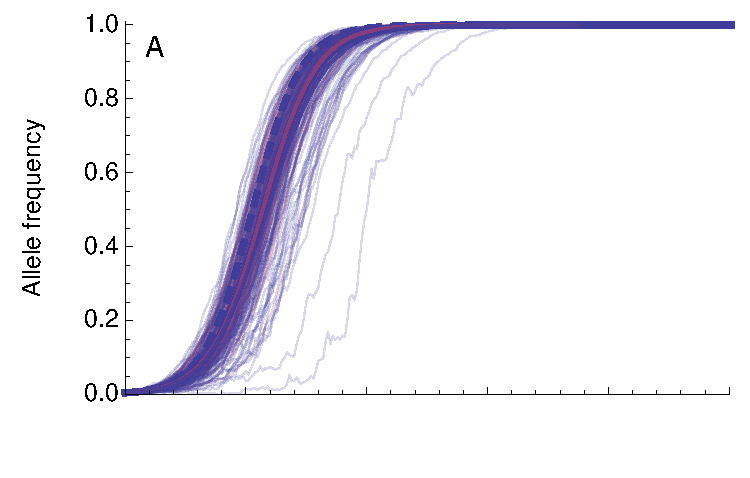
\includegraphics[width=0.49\linewidth]{pt_rescue_s0.2_k100_u0_m0.pdf}};
\node[below = -1cm of A1] (A2) {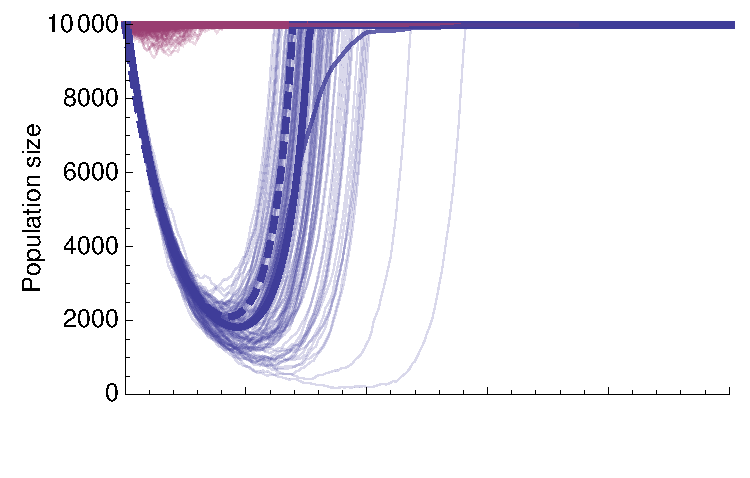
\includegraphics[width=0.49\linewidth]{nt_rescue_s0.2_k100_u0_m0.pdf}};
\node[right = 0cm of A1] (B1) {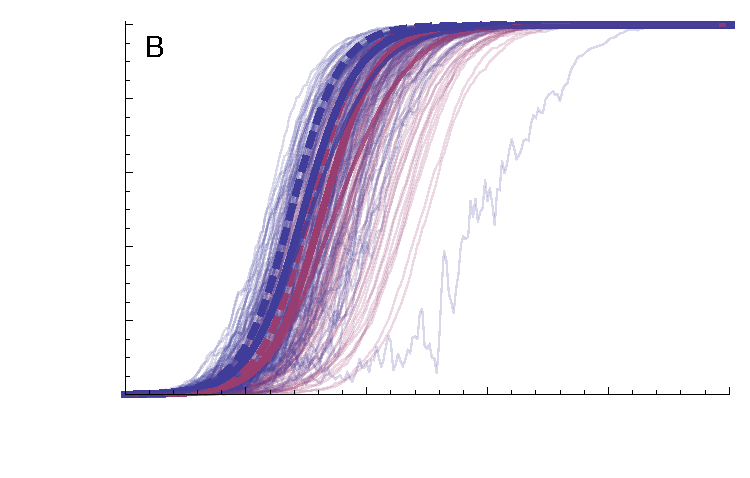
\includegraphics[width=0.49\linewidth]{pt_rescue_s0.2_k1_u0_m0.pdf}};
\node[right = 0cm of A2] (B2) {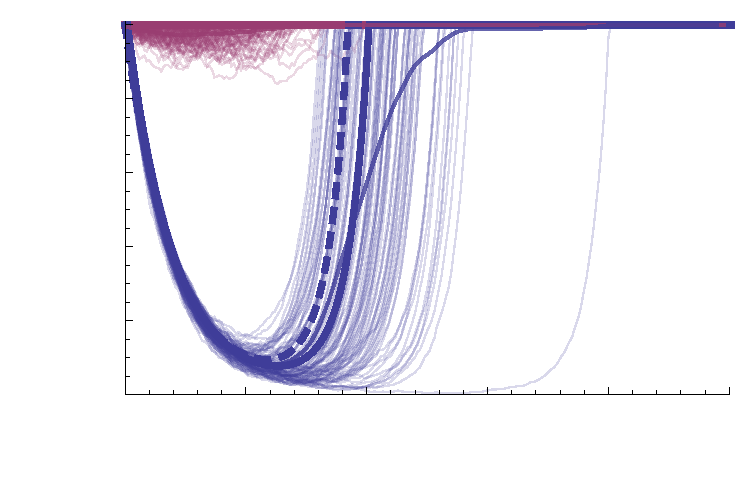
\includegraphics[width=0.49\linewidth]{nt_rescue_s0.2_k1_u0_m0.pdf}};
\node[below = 0cm of A2] (C1) {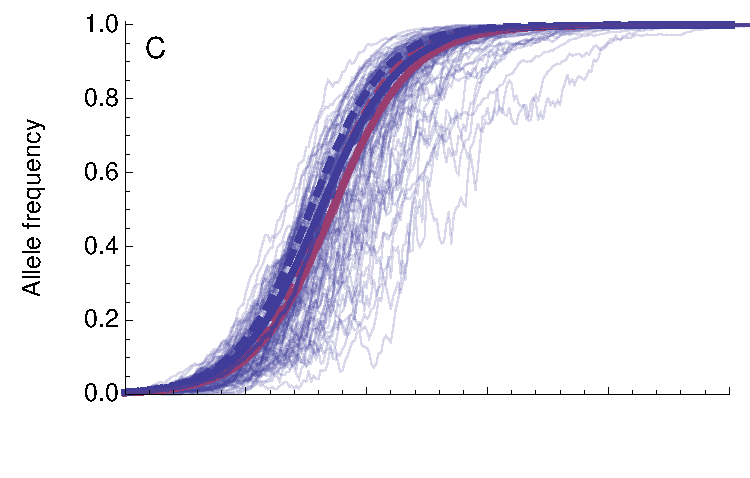
\includegraphics[width=0.49\linewidth]{pt_rescue_s0.13_k100_u0_m0.pdf}};
\node[below = -1cm of C1] (C2) {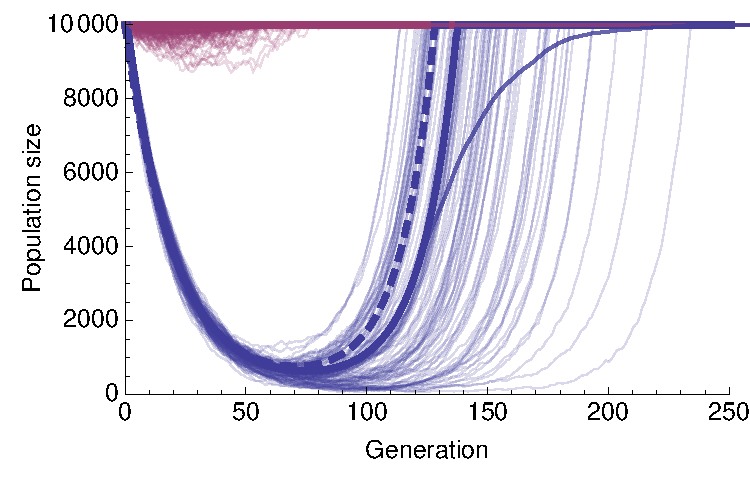
\includegraphics[width=0.49\linewidth]{nt_rescue_s0.13_k100_u0_m0.pdf}};
\node[right = 0cm of C1] (D1) {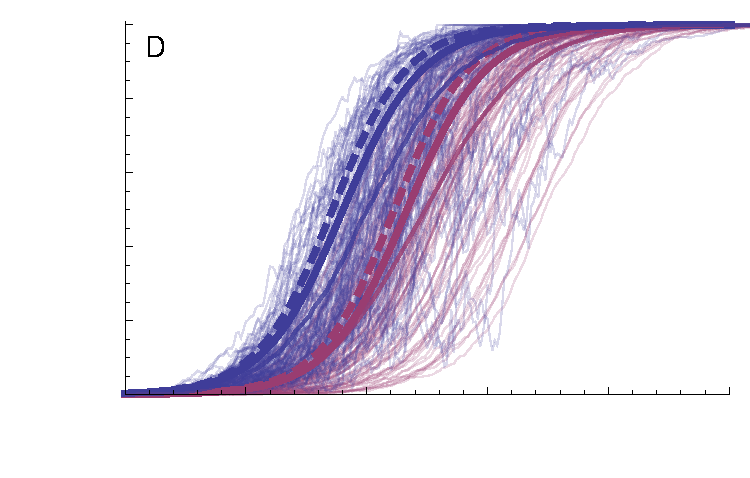
\includegraphics[width=0.49\linewidth]{pt_rescue_s0.13_k1_u0_m0.pdf}};
\node[right = 0cm of C2] (D2) {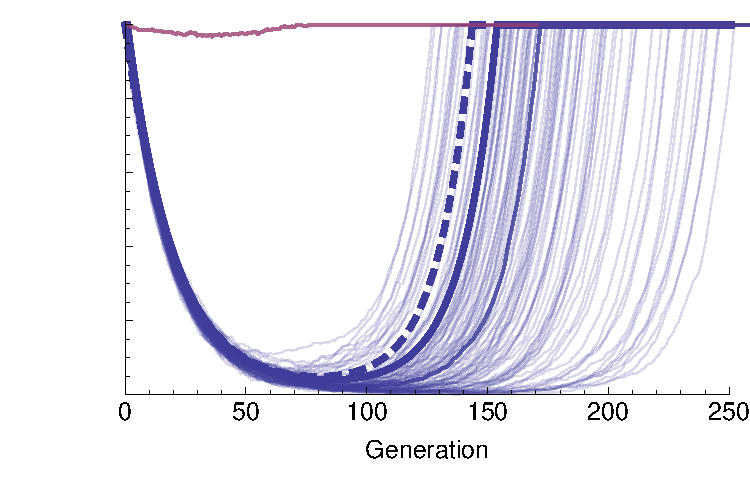
\includegraphics[width=0.49\linewidth]{nt_rescue_s0.13_k1_u0_m0.pdf}};
\node[right = 0.5 of A1, yshift = -2.5cm, rotate = 90, draw, rectangle, rounded corners, thick, fill=gray!50] (s) {\large$\bm{s=0.20}$};
\node[right = 0.5 of C1, yshift = -2.5cm, rotate = 90, draw, rectangle, rounded corners, thick, fill=gray!50] {\large$\bm{s=0.13}$};
\node[below = -0.6cm of A2, xshift = 20, draw, rectangle, rounded corners, thick, fill=gray!50] (k) {\large$\bm{\kappa=100}$};
\node[below = -0.6cm of B2, xshift = 20, draw, rectangle, rounded corners, thick, fill=gray!50] {\large$\bm{\kappa=1}$};
\node[right = 2cm of k, darkred, yshift = 0.25cm, draw, rectangle, rounded corners, thick, fill=darkred!25] (N) {\fontfamily{phv}\selectfont\textbf{constant $\bm{N}$}};
\node[below = 0cm of N, darkblue, draw, rectangle, rounded corners, thick, fill=darkblue!25] {\fontfamily{phv}\selectfont\textbf{evol.\ rescue}};
\end{tikzpicture}
\caption{
Allele frequency, $p(t)$, and population size, $N(t)$, during a selective sweep from standing genetic variance in evolutionary rescue (blue; $d=0.05$) or in a population of roughly constant size (red; $d=0$ such that $\mathbb{E}[N(t)]=N(0)$, not shown).
The thick solid curves are the numerical predictions (Equation \ref{eq:deltapdeltaN}) and the dashed curves are the analytic approximations (Equation \ref{eq:ptnt}), after replacing the true initial allele frequency, $p(0)=\kappa/[2N(0)]$ with $p_{0|\mathrm{rescue}}^{\mathrm{SGV}}$ (Equation \ref{eq:p0sgv}).
%The thick red curves are hidden by the thick blue curves in panel A.
The thinnest curves are 100 replicate simulations (rescue only for clarity), with the median trajectory slightly thicker (often obscured by predictions).
}%
\label{fig:rescueSGV_dynamics}
\end{figure}
%%%%%%%%%%%%%%%%%%%%%%%%%%%%%%%%%%%%%%%%%%%%%%%

Note that when the expected number of establishing copies, $\rho \kappa$, is small, the probability of rescue is roughly $\rho \kappa$, so that the effective initial allele frequency, $p_{0|\mathrm{rescue}}^{\mathrm{SGV}}$, is independent of the initial number of copies, $\kappa$, implying that rescue tends to occur by a hard selective sweep, i.e., only one of the initial copies establishes.
For larger values of $\kappa$ the effective initial frequency is not independent of $\kappa$ and rescue can occur by a soft selective sweep \citep{hermisson2005soft}, where multiple initial copies establish.
The probability that multiple copies establish is $P^\mathrm{SGV}_\mathrm{rescue} - \kappa \rho (1-\rho)^{\kappa-1}$, where $\kappa \rho (1-\rho)^{\kappa-1}$ is the probability of a hard sweep.
Given rescue occurs from standing genetic variation, the probability it is due to a soft sweep is therefore 
\begin{equation}\label{eq:PsoftSGV}
P_{\mathrm{soft}|\mathrm{rescue}}^{\mathrm{SGV}} = 1 - \frac{\kappa \rho}{1-\rho}\frac{1-P_{\mathrm{rescue}}^{\mathrm{SGV}}}{P_{\mathrm{rescue}}^{\mathrm{SGV}}}.
\end{equation}
In our two examples above this is 0 (when $\kappa=1$) and $\approx1$ (when $\kappa=100$).
Between these two extremes we find Equation \ref{eq:PsoftSGV} to provide reasonable estimates for small $\kappa$ or large $s$, but to underestimate the probability of a soft sweep otherwise (Figure \ref{fig:PsoftSGV}A), when beneficial alleles can persist at low numbers long enough to establish with some non-negligible probability of experiencing some selection as homozygotes (given $d>0$).

More generally, as mentioned above, the number that establish is binomially distributed, and dividing this by the probability of rescue then provides the distribution given rescue, which has expectation 
\begin{equation}\label{eq:ENestSGV}
\mathbb{E}[\mathrm{number\; of\; copies\; that\; establish}|\mathrm{rescue}] = \frac{\kappa \rho}{P^\mathrm{SGV}_\mathrm{rescue}}.
\end{equation}
Equation \ref{eq:ENestSGV} also provides reasonable estimates for small $\kappa$ or large $s$ (Figure \ref{fig:PsoftSGV}B).

%%%%%%%%%%%%%%%%%%%%%%%%%%%%%%%%%%%%%%%%%%%%%%%
\begin{figure}[htb]
\centering
\begin{tikzpicture}
\node[] (A) {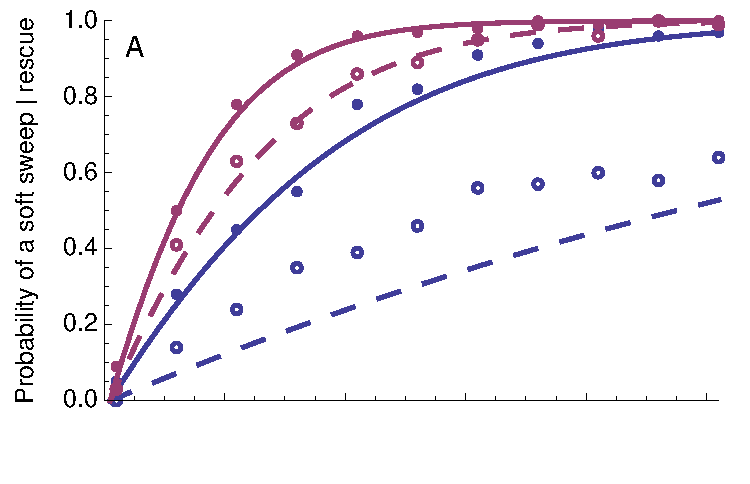
\includegraphics[width=0.49\linewidth]{PsoftSGV.pdf}};
\node[below = -1cm of A] (B) {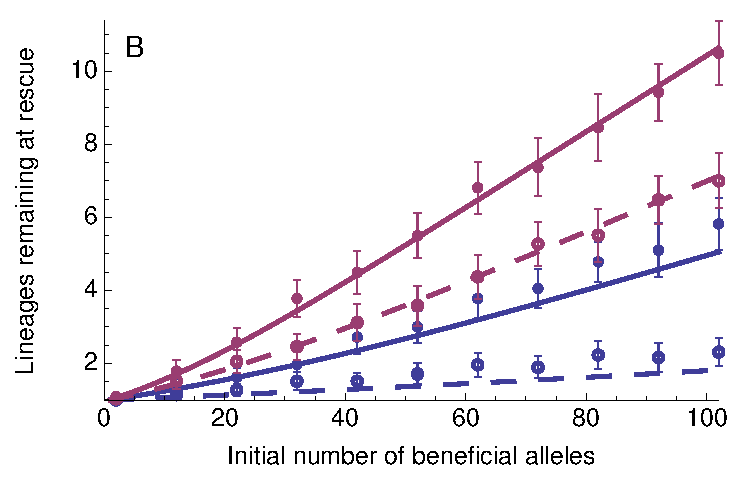
\includegraphics[width=0.49\linewidth]{NumberEstSGV.pdf}};
\node[below = -1cm of A, xshift = -0.75cm, darkred, draw, rectangle, rounded corners, thick, fill=darkred!25] (N) {\fontfamily{phv}\selectfont\textbf{constant $\bm{N}$}};
\node[right = 0cm of N, darkblue, draw, rectangle, rounded corners, thick, fill=darkblue!25] {\fontfamily{phv}\selectfont\textbf{evol.\ rescue}};
\draw[very thick] (-1,-2.5) -- (-0.25,-2.5); 
\draw[fill=black] (0,-2.5) circle (0.05cm);
\node at (0.75, -2.475) {$s=0.2$}; 
\draw[very thick] (-1,-2.9) -- (-0.75,-2.9); \draw[very thick] (-0.5,-2.9) -- (-0.25,-2.9); 
\draw[very thick] (0,-2.9) circle (0.05cm);
\node at (0.84, -2.875) {$s=0.13$}; 
\end{tikzpicture}
\caption{
(A) The probability more than one initial copy of the beneficial allele establishes given rescue (blue; $d=0.05$) or fixation (red; $d=0$) and (B) the expected number of initial copies that have descendants at the time of rescue (or fixation), each as functions of the initial number of copies of the beneficial allele, $\kappa$.
The curves are Equations \ref{eq:PsoftSGV} (panel A) and \ref{eq:ENestSGV} (panel B).
Each point is based on 100 replicate simulations where rescue (or fixation) was observed.
Error bars are standard errors.
Parameters: $N(0)=10^4$.
}%
\label{fig:PsoftSGV}
\end{figure}
%%%%%%%%%%%%%%%%%%%%%%%%%%%%%%%%%%%%%%%%%%%%%%%

%%%%%%%%%%%%%%%%%%%%%%%%%%%%%%%%%%%%%%%%%%%%%%%%%%%
\subsubsection*{Rescue by \textit{de novo} mutation (DNM)}
\label{sec:rescue_forward_DNM}

When there are few copies of the beneficial allele at the time of environmental change rescue may depend on mutations arising \textit{de novo} at the selected site during population decline.
To predict the allele frequency and population size dynamics in this scenario we then need to derive the waiting time until the first successful rescue mutation.
The first successful rescue mutation arrives according to a time-inhomogeneous Poisson process with rate, $\lambda(t) = 2 N(t) u \rho$, where $2N(t) = 2N(0) e^{-d t}$ describes the decline in the number of copies of the ancestral allele.
Thus the probability that a rescue mutation has established by time $T$ (i.e., the cumulative distribution of the waiting time) is $F(T) = 1-e^{-\int_0^T \lambda(t) \mathrm{d}t}$.
Taking the limit as time goes to infinity then gives the probability of rescue \citep[c.f., equation 10 in][]{orr2008population}
\begin{equation}
P_{\mathrm{rescue}}^{\mathrm{DNM}} = \lim_{T\rightarrow\infty} F(T) = 1 - e^{-2 N(0) u \rho / d}.
\end{equation}
Following \cite{orr2014population}, taking the derivative of $F(T)$ and dividing by the probability of rescue gives the probability distribution function for the arrival time of the first establishing rescue mutation given rescue, $f(t)$.
While the first establishing mutation is still rare it will grow exponentially at rate $\rho/2$, and conditioned on its establishment will very quickly reach $1/\rho$ copies. 
Integrating over the possible arrival times then gives the expected number of copies of this successful mutation at time $t$ since the environmental change, $\int_0^\infty (e^{(t-\tau) \rho/2} / \rho) f(\tau) \mathrm{d}\tau$.
Dividing by its expected size at time $t$, $\exp(\rho t/2)$, and the total number of alleles at the time of environmental change, $2N(0)$, it is therefore as if the successful mutation was present at the time of environmental change, with frequency
\begin{equation}\label{eq:p0dnm}
p_{0|\mathrm{rescue}}^{\mathrm{DNM}} = \frac{1}{2N(0)}\frac{1}{\rho}\frac{(-2N(0) u \rho/d)^{-\rho/(2d)} \left[\Gamma(1+\rho/(2d),-c) - \Gamma(1+\rho/(2d)) \right]}{1-\exp(2N(0) u \rho/d)},
\end{equation}
where $\Gamma(z)$ is the gamma function \citep[equation 6.1.1 in][]{abramowitz1972handbook} and $\Gamma(a,x)$ is the incomplete gamma function \citep[equation 6.5.3 in][]{abramowitz1972handbook}.
The factor $1/\rho>1$ increases the effective initial frequency, because we have conditioned on establishment, while the last factor decreases the effective initial frequency, because we must wait for the mutation to arise.
When the expected number of rescue mutations, $ 2 u N(0) \rho / d$, is small this expected number cancels out and the last factor becomes approximately $d/(d+\rho/2)$, which is independent of mutational input \citep{orr2014population}.
That is, conditioning on unlikely rescue, rescue mutations arise earlier in populations that decline faster.

In a population of constant size, $N=N(0)$, mutations arrive at a time-homogeneous rate, $\lambda=2 N(0) u \rho$ and the probability distribution of the waiting time until the first successful mutation is a simple exponential, $f(t) = \lambda e^{-\lambda t}$.
Integrating the expected number of copies of the allele over the waiting times shows that the waiting time factor in a population of roughly constant size is $4N(0)u/(1+4N(0)u)$, which, in constrast to rescue, depends strongly on mutational input but is independent of establishment probability, $\rho$.

Figure \ref{fig:rescueDNM_dynamics} compares our numerical (Equation \ref{eq:deltapdeltaN}) and analytical (Equations \ref{eq:ptnt}) approximations against individual-based simulations.
As with rescue from standing genetic variance (Figure \ref{fig:rescueSGV_dynamics}), with small selection coefficients we tend to overestimate allele frequencies and population sizes by ignoring beneficial homozygotes and thus underestimating of the probability of establishment.
This is an even bigger issue with rescue by \textit{de novo} mutation, where a weakly selected beneficial allele can not only exist at low numbers for a large number of generations before establishing, but can also arise when the number of ancestral alleles is already considerably lowered (especially so when the mutation rate is small).
Our predictions do better with larger selection coefficients, where beneficial alleles quickly establish or go extinct.

%%%%%%%%%%%%%%%%%%%%%%%%%%%%%%%%%%%%%%%%%%%%%%%
\begin{figure}[htbp]
\centering
\begin{tikzpicture}
\node[] (A1) {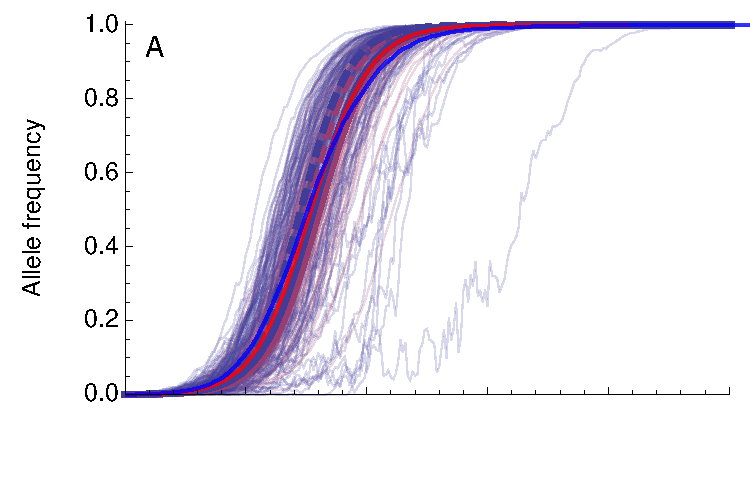
\includegraphics[width=0.49\linewidth]{pt_rescue_s0.2_k0_u0.0001_m0.pdf}};
\node[below = -1cm of A1] (A2) {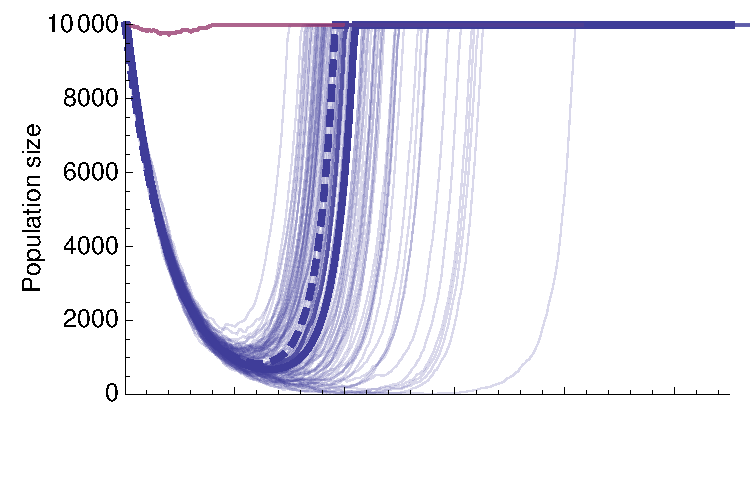
\includegraphics[width=0.49\linewidth]{nt_rescue_s0.2_k0_u0.0001_m0.pdf}};
\node[right = 0cm of A1] (B1) {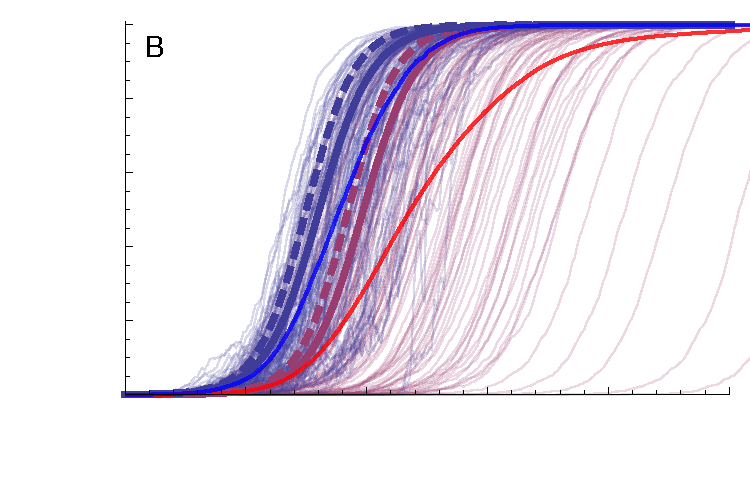
\includegraphics[width=0.49\linewidth]{pt_rescue_s0.2_k0_u0.00001_m0.pdf}};
\node[right = 0cm of A2] (B2) {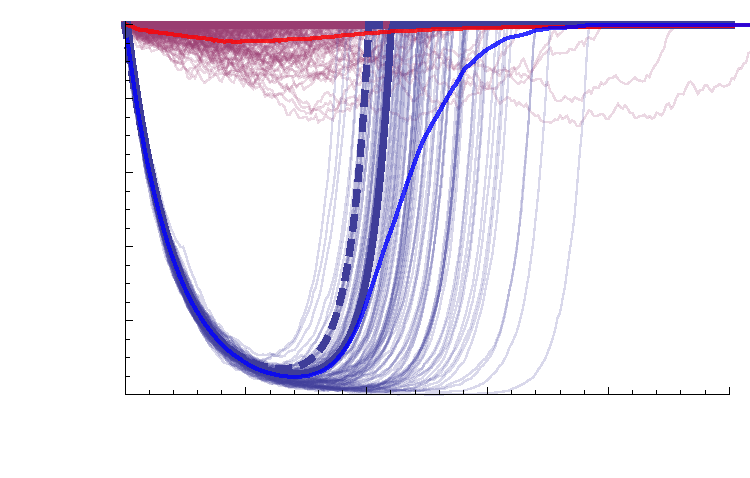
\includegraphics[width=0.49\linewidth]{nt_rescue_s0.2_k0_u0.00001_m0.pdf}};
\node[below = 0cm of A2] (C1) {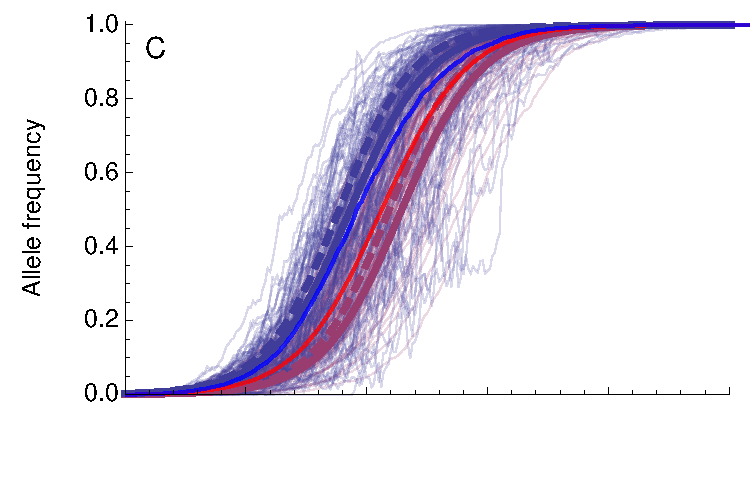
\includegraphics[width=0.49\linewidth]{pt_rescue_s0.13_k0_u0.0001_m0.pdf}};
\node[below = -1cm of C1] (C2) {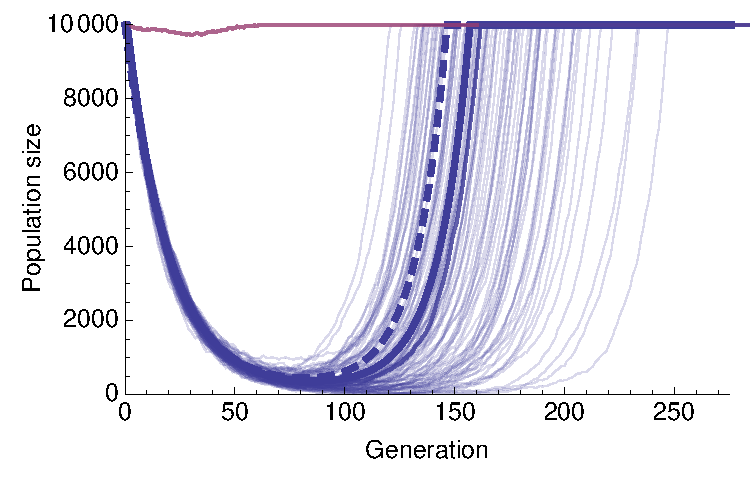
\includegraphics[width=0.49\linewidth]{nt_rescue_s0.13_k0_u0.0001_m0.pdf}};
\node[right = 0cm of C1] (D1) {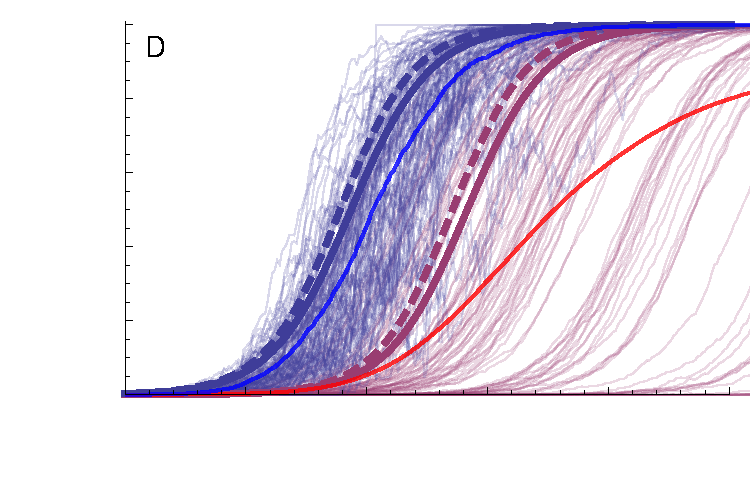
\includegraphics[width=0.49\linewidth]{pt_rescue_s0.13_k0_u0.00001_m0.pdf}};
\node[right = 0cm of C2] (D2) {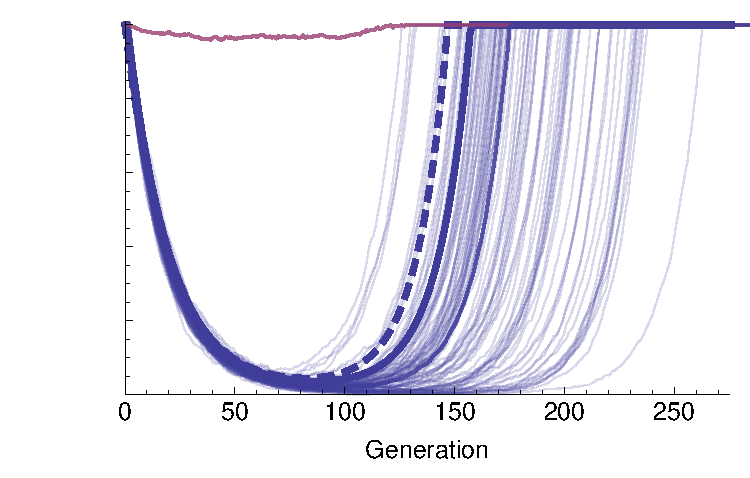
\includegraphics[width=0.49\linewidth]{nt_rescue_s0.13_k0_u0.00001_m0.pdf}};
\node[right = 0.5 of A1, yshift = -2.5cm, rotate = 90, draw, rectangle, rounded corners, thick, fill=gray!50] (s) {\large$\bm{s=0.20}$};
\node[right = 0.5 of C1, yshift = -2.5cm, rotate = 90, draw, rectangle, rounded corners, thick, fill=gray!50] {\large$\bm{s=0.13}$};
\node[below = -0.6cm of A2, xshift = 20, draw, rectangle, rounded corners, thick, fill=gray!50] (k) {\large$\bm{u=10^{-4}}$};
\node[below = -0.6cm of B2, xshift = 20, draw, rectangle, rounded corners, thick, fill=gray!50] {\large$\bm{u=10^{-5}}$};
\node[right = 2cm of k, darkred, yshift = 0.25cm, draw, rectangle, rounded corners, thick, fill=darkred!25] (N) {\fontfamily{phv}\selectfont\textbf{constant $\bm{N}$}};
\node[below = 0cm of N, darkblue, draw, rectangle, rounded corners, thick, fill=darkblue!25] {\fontfamily{phv}\selectfont\textbf{evol.\ rescue}};
\end{tikzpicture}
\caption{
Allele frequency, $p(t)$, and population size, $N(t)$, during a selective sweep from \textit{de novo} mutation in evolutionary rescue (blue; $d=0.05$) and in a population of roughly constant size (red; $d=0$).
The thick solid curves are the numerical predictions (Equation \ref{eq:deltapdeltaN}) and the dashed curves are the analytic approximations (Equation \ref{eq:ptnt}), using $p_{0|\mathrm{rescue}}^{\mathrm{DNM}}$ (Equation \ref{eq:p0dnm}) as the initial allele frequency, $p(0)$.
See Figure \ref{fig:rescueSGV_dynamics} for details.
}%
\label{fig:rescueDNM_dynamics}
\end{figure}
%%%%%%%%%%%%%%%%%%%%%%%%%%%%%%%%%%%%%%%%%%%%%%%%

We can also calculate the probability of a soft sweep from recurrent mutation.
Taking into account the beneficial alleles present at time $t$, the rate at which additional copies arise and establish is $\lambda(t) = 2 N(t) q(t) u \rho(t)$, where $2 N(t) q(t)$ is the number of ancestral alleles at time $t$ and $\rho(t)$ is the probability of establishment, which changes with allele frequency because this influences the genotypes the new allele experiences.
Thus the number of mutations that arise and fix is Poisson with rate $\int_0^\infty \lambda(t) \mathrm{d} t$, allowing us to write down an equation for the probability of a soft sweep. 
To gain intuition we make a very rough approximation, assuming $q(t)\approx1$ while mutations are arriving (i.e., when $N(t)$ is still large), so that $\rho(t)\approx\rho$ and we get the same Poisson rate we derived above for the first successful mutation, $\int_0^\infty \lambda(t) \mathrm{d} t \approx 2N(0) u \rho/d$, providing us with the probability distribution for the number of mutations that establish.
Dividing the expected number of establishing mutations by the probability of rescue, the expected number that establish given rescue is
\begin{equation}\label{eq:ENestDNM}
\mathbb{E}[\mathrm{number\; of\; mutations\; that\; establish}|\mathrm{rescue}] = P_\mathrm{rescue}^\mathrm{DNM} + \log(1-P_\mathrm{rescue}^\mathrm{DNM})(1-P_\mathrm{rescue}^\mathrm{DNM}).
\end{equation}
This is analogous to the result in a model with haploid selection \citep[c.f., equation 7 in][]{wilson2017soft}.  
Ignoring density-dependence, our approximation will underestimate the number of establishing mutations when $h\neq0$ since selection in heterozygotes will prolong the persistence of the $a$ allele (creating more opportunity for mutation) and establishment probabilities will rise with the frequency of the beneficial $A$ allele (because more $AA$ genotypes are then created, as discussed in the case of standing genetic variation above).
At the same time, if the carrying capacity is reached before fixation, our simple form of density-dependence will introduce additional genetic drift and hence tend to reduce the number of mutations that establish.
In the end we find our rough approximation to underestimate the number of establishing mutations (Figure \ref{fig:PsoftDNM}B), suggesting that our underestimate of the probability of establishment has a larger effect than the excess drift brought about by the carrying capacity for these parameter values.

With these same approximations the probability of a soft selective sweep given rescue (i.e., the probability more than one copy establishes) is 
\begin{equation}\label{eq:PsoftDNM}
P_{\mathrm{soft}|\mathrm{rescue}}^{\mathrm{DNM}} = 1 + \log(1-P_\mathrm{rescue}^\mathrm{DNM}) \frac{1-P_{\mathrm{rescue}}^{\mathrm{DNM}}}{P_{\mathrm{rescue}}^{\mathrm{DNM}}},
\end{equation}
as in a haploid population \citep[equation 8 in][]{wilson2017soft}.
As with the expected number of establishing copies (Equation \ref{eq:ENestDNM}), we see this approximation is an underestimate in diploid populations (Figure \ref{fig:PsoftDNM}A).
On a related note, \cite{wilson2017soft} reasoned that, because soft sweeps are expected when rescue is likely while hard sweeps are expected when rescue is rare, population bottlenecks will tend to be more extreme when rescue occurs by a hard selective sweep (and thus it might be easier to detect soft sweeps from patterns at linked neutral loci, as bottlenecks could hide the signal).
Here we show the importance of conditioning on rescue, which roughly equalizes the bottleneck sizes across scenarios with very different probabilities of rescue (e.g., compare Figure \ref{fig:rescueDNM_dynamics}A and B, or C and D, where the probability of rescue differs by an order of magnitude), potentially making hard sweeps easier to detect due to their greater effect on local gene genealogies (see below).

%%%%%%%%%%%%%%%%%%%%%%%%%%%%%%%%%%%%%%%%%%%%%%%
\begin{figure}[htb]
\centering
\begin{tikzpicture}
\node[] (A) {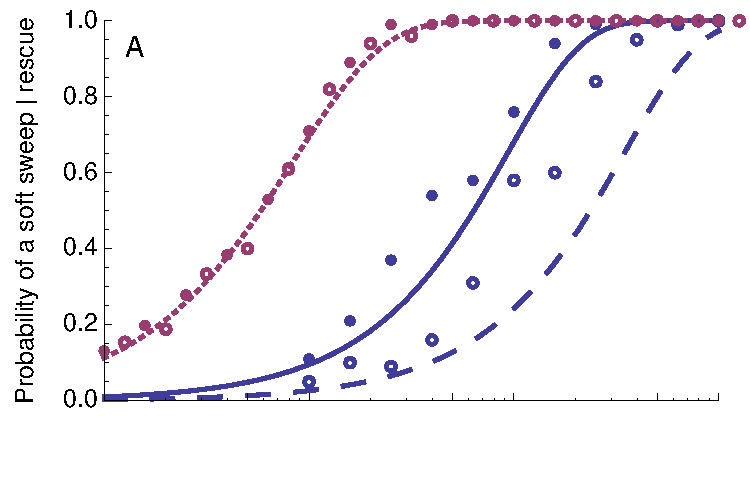
\includegraphics[width=0.49\linewidth]{PsoftDNM.pdf}};
\node[below = -1cm of A] (B) {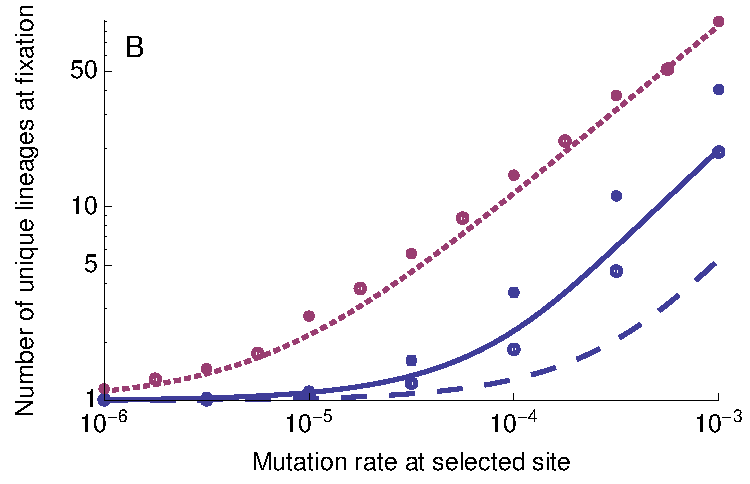
\includegraphics[width=0.49\linewidth]{NumberEstDNM.pdf}};
\node[below = -1cm of A, xshift = -0.75cm, darkred, draw, rectangle, rounded corners, thick, fill=darkred!25] (N) {\fontfamily{phv}\selectfont\textbf{constant $\bm{N}$}};
\node[right = 0cm of N, darkblue, draw, rectangle, rounded corners, thick, fill=darkblue!25] {\fontfamily{phv}\selectfont\textbf{evol.\ rescue}};
\draw[very thick] (-1,-2.5) -- (-0.25,-2.5); 
\draw[fill=black] (0,-2.5) circle (0.05cm);
\node at (0.75, -2.475) {$s=0.2$}; 
\draw[very thick] (-1,-2.9) -- (-0.75,-2.9); \draw[very thick] (-0.5,-2.9) -- (-0.25,-2.9); 
\draw[very thick] (0,-2.9) circle (0.05cm);
\node at (0.84, -2.875) {$s=0.13$}; 
\end{tikzpicture}
\caption{
(A) The probability more than one mutation establishes given rescue (blue; $d=0.05$) or fixation (red; $d=0$) and (B) the expected number of unique mutational lineages of the beneficial allele that exist at the time of rescue (or fixation), each as functions of the mutation rate at the selected locus, $u$.
The blue curves are Equations \ref{eq:PsoftDNM} (panel A) and \ref{eq:ENestDNM} (panel B).
The red curves are from Ewens' sampling formula \citep[equation 11 (panel A) and equation 12 (panel B) in ][with $\theta = 2N_e(0) u = 8 N(0) u/7$ and $n=2N(0)$]{pennings2006soft2}.
Each point is based on 100 replicate simulations where rescue (or fixation) was observed.
Error bars are standard errors.
Parameters: $N(0)=10^4$.
}%
\label{fig:PsoftDNM}
\end{figure}
%%%%%%%%%%%%%%%%%%%%%%%%%%%%%%%%%%%%%%%%%%%%%%%

%%%%%%%%%%%%%%%%%%%%%%%%%%%%%%%%%%%%%%%%%%%%%%%%%%%
\subsubsection*{Rescue by migrant alleles (MIG)}
\label{sec:rescue_forward_mig_main}

In \nameref{sec:rescue_forward_mig} we derive approximations for allele frequency and population size dynamics given rescue by migrant alleles entering the population at a constant per generation rate $m$.
There are close similarities here with rescue by mutation, and so we largely relegate this case to the appendix.
However, with migration as opposed to mutation, the rate at which new copies of the beneficial allele arise does not decline with the number of ancestral alleles.
This increases the probability that beneficial alleles will establish when the population is closer to extinction, when compared to rescue by mutation, especially under smaller migration rates.
This effect is amplified by the fact that the probability of establishment also increases as the number of ancestral alleles declines.
Under sufficiently small migration rates, simulations show that the beneficial allele starts to sweep later but increases in frequency faster than the deterministic expectation (Figure \ref{fig:rescueMIG_dynamics}).
Here we enter a different regime, which we do not explore.

We wait until the coalescent has been introduced to explore soft sweeps under migration (see \nameref{sec:ewens_migrants}).

%%%%%%%%%%%%%%%%%%%%%%%%%%%%%%%%%%%%%%%%%%%%%%%%%%%
\subsection*{The structured coalescent}
\label{sec:rescue_backward}

To explore the genetic patterns created by evolutionary rescue we next flip our perspective and think backwards in time, starting from a random sample of chromosomes at the time the beneficial allele fixes.
Focusing on a neutral locus that is recombination distance $r$ from the selected site, we are interested in calculating the rate of coalescence, the rates of recombination and mutation off the selected background, and the rate of migration out of the population.
If our sample of alleles has $k$ distinct ancestors on the selected background $\tau$ generations before fixation, these rates are approximately (table 1 in \citealp{hudson1988coalescent}; equation 16 in \citealp{pennings2006soft2}; see \nameref{sec:derive_coalescent} for derivations)
\begin{equation}\label{eq:coal_rates}
\begin{aligned}
p_{\mathrm{coal}}(k,\tau) &= \binom{k}{2} \frac{1}{2N_e'(\tau) p'(\tau)}\\
p_{\mathrm{rec}}(k,\tau) &= k r [1 - p'(\tau)]\\
p_{\mathrm{mut}}(k,\tau) &= k \frac{u [1 - p'(\tau)]}{p'(\tau)}\\
p_{\mathrm{mig}}(k,\tau) &= k \frac{m}{2N'(\tau)p'(\tau)},
\end{aligned}
\end{equation} 
where $p'(\tau) = p(T - \tau)$, $N'(\tau)=N(T-\tau)$, and $N_e'(\tau) = N_e(T - \tau)$ are the allele frequency, census population size, and effective population size, respectively, $\tau$ generations before fixation, with fixation occurring in generation $T$.

With slow changes in population size, $N(t-1)\approx N(t)$ and the mean number of gametes contributed to the next generation by each gamete in the current generation is $2$.
The inbreeding (and variance) effective population size, $N_e(t)$, is then roughly $(4N(t) - 2)/(\sigma^2+2)$ \citep[equation 7.6.4.3 in][]{crow1970introduction}, where $\sigma^2$ is the variance in the per capita number of gametes contributed to the next generation.
Therefore, in a large population, $N(t)\gg1$, the ratio of the effective size to the census size is roughly
\begin{equation}\label{eq:Ne}
\frac{N_e(t)}{N(t)} \approx \frac{4}{2+\sigma^2},
\end{equation}
where $\sigma^2$ depends on the particular lifecycle (e.g., see \nameref{sec:pestNe}). 

%%%%%%%%%%%%%%%%%%%%%%%%%%%%%%%%%%%%%%%%%%%%%%%%%%%
\subsubsection*{The number of successful migrants}
\label{sec:ewens_migrants}

Before moving on, note that Equation \ref{eq:coal_rates} (together with Equation \ref{eq:Ne} when $\sigma^2$ is constant) shows that the per generation probability of migration and coalescence depend on population size and beneficial allele frequency in the same way. 
This similar form implies that the relative rates at which lineages coalesce and migrate at the selected site does not depend on the population size and allele frequency. 
\cite{pennings2006soft2} used this fact to show that, in an ideal population of constant size, the number of unique migrant haplotypes contributing to a present day sample, as well as their proportions, is described by Ewens' sampling formula \citep[pages 334\textit{ff} in][]{ewens2004mathematical} when we replace $\theta$ with $2 m$. 
Powerfully, this results holds even in non-ideal populations of changing size \citep[as briefly noted by][p.\ 1081-1082]{pennings2006soft2} -- including during evolutionary rescue -- as long as the relationship between the effective and census population sizes remains the same (i.e., $N_e(t)/N(t)$ is constant; we now replace $\theta$ with $2m N_e/N$ in Ewens' sampling formula). 
Thus the softness of a sweep from migration depends only on the migration rate and variance in gamete numbers ($\sigma^2$, which determines $N_e/N$; Equation \ref{eq:Ne}), and is the same during rescue as it is in a population of constant size.
The analogous result for rescue by \textit{de novo} mutation does not hold \citep[as it does for a population of constant size,][]{pennings2006soft2}, since the rate of mutation is not inversely proportional to population size (Equation \ref{eq:coal_rates}).  

Here we use just two properties of Ewens' sampling formula, the expected number of unique migrants among a sample of size $n$ \citep[page 336 in][]{ewens2004mathematical}
\begin{equation}\label{eq:ewens_number}
\mathbb{E}[\mathrm{number\; of\; unique\; migrants\;} | n] = \sum_{j=1}^n \frac{2 m N_e/N}{j - 1 + 2 m N_e/N}
\end{equation}
and the probability this is more than two is \citep[equation 10.9 in][]{ewens2004mathematical}
\begin{equation}\label{eq:ewens_Psoft}
P_{\mathrm{soft}|\mathrm{rescue}}^\mathrm{MIG}(n) = 1 - \prod_{j=1}^{n-1} \frac{j}{j + 2 m N_e/N}.
\end{equation}
Figure \ref{fig:PsoftMIG} shows that these formulas perform very well, even when we sample the entire population ($n=2N(0)$).

%%%%%%%%%%%%%%%%%%%%%%%%%%%%%%%%%%%%%%%%%%%%%%%
\begin{figure}[htb]
\centering
\begin{tikzpicture}
\node[] (A) {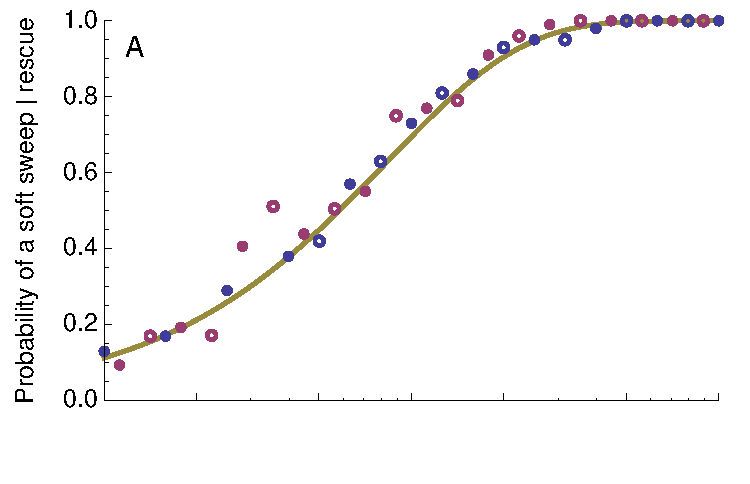
\includegraphics[width=0.49\linewidth]{PsoftMIG.pdf}};
\node[below = -1cm of A] (B) {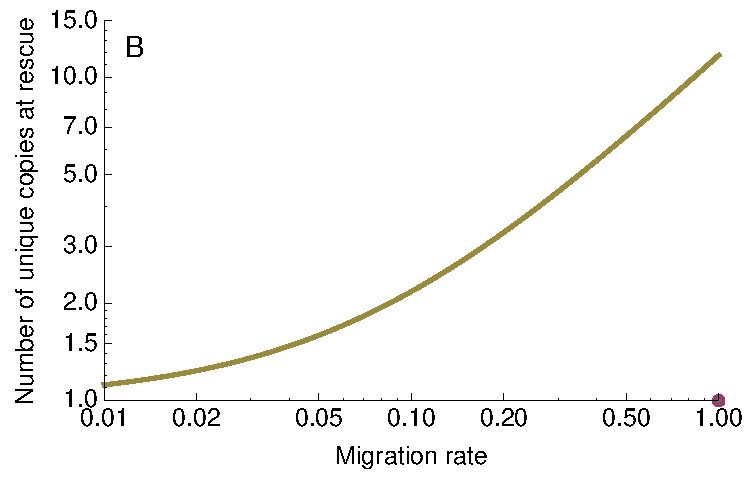
\includegraphics[width=0.49\linewidth]{NumberEstMIG.pdf}};
\node[below = -1cm of A, xshift = -0.75cm, darkred, draw, rectangle, rounded corners, thick, fill=darkred!25] (N) {\fontfamily{phv}\selectfont\textbf{constant $\bm{N}$}};
\node[right = 0cm of N, darkblue, draw, rectangle, rounded corners, thick, fill=darkblue!25] {\fontfamily{phv}\selectfont\textbf{evol.\ rescue}};
\draw[fill=black] (0,-2.5) circle (0.05cm);
\node at (0.75, -2.475) {$s=0.2$}; 
\draw[very thick] (0,-2.9) circle (0.05cm);
\node at (0.84, -2.875) {$s=0.13$}; 
\end{tikzpicture}
\caption{
(A) The probability that more than migrant allele establishes given rescue ($d=0.05$; blue) or fixation ($d=0$; red) and (B) the expected number of unique lineages of the beneficial allele that exist at the time of rescue (or fixation), each as functions of the migration rate, $m$.
The yellow curves are Equations \ref{eq:ewens_Psoft} (panel A) and \ref{eq:ewens_number} (panel B) using $n=2N(0)$.
Each point is based on 100 replicate simulations where rescue (or fixation) was observed.
Error bars are standard errors.
Parameters: $N(0)=10^4$.
}%
\label{fig:PsoftMIG}
\end{figure}
%%%%%%%%%%%%%%%%%%%%%%%%%%%%%%%%%%%%%%%%%%%%%%%

%%%%%%%%%%%%%%%%%%%%%%%%%%%%%%%%%%%%%%%%%%%%%%%%%%%
\subsubsection*{The timing of coalescence}

We now use Equation \ref{eq:coal_rates} to calculate the probability that the most recent event is $\tau$ generations before fixation and is either coalescence, recombination, mutation, or migration. 
Letting $i,j\in\{\mathrm{coal, rec, mut, mig}\}$, the probability that $i$ is the most recent event, and occurs $\tau$ generations before fixation, is \citep[c.f., equation 6 in][]{pennings2006soft}
\begin{equation}\label{eq:Pikt}
\begin{aligned}
P_{i}(k,\tau) &= p_{i}(k,\tau) \left( \prod_{j\neq i} [1 - p_{j}(k,\tau)] \right) \prod_{l=0}^{\tau-1} \left( \prod_{j} [1 - p_{j}(k,l)] \right)\\
&\approx p_{i}(k,\tau) \exp \left( -\sum_{j} \int_{0}^{\tau} p_{j}(k,l) \mathrm{d}l \right),
\end{aligned}
\end{equation}
i.e., the waiting time for an inhomogeneous exponential random variable.
The approximation assumes the $p_i(k,\tau)$ are small enough such that at most one event happens each generation, with small probability, and the changes in the $p_i(k,\tau)$ from one generation to the next are small enough that we can approximate a sum across $\tau$ with an integral.
As a technical aside, to speed computation we analytically solve the integrals and then numerically evaluate Equation \ref{eq:Pikt} under the assumption of weak selection and exponential population growth (Equation \ref{eq:ptnt}); in contrast, the simulations impose a hard carrying capacity of $N(0)$, creating a discrepancy when the bottleneck is finished long before the sweep ($d\ll s \ll1$).
The fixation time, $T$, is approximated by solving $p(T) = 1-1/[2N(0)]$ using Equation \ref{eq:ptnt}, and thus also assumes weak selection.

Figures \ref{fig:rescueSGV_timing}--\ref{fig:rescueDNM_timing} and \ref{fig:rescueMIG_timing} show the probability and timing of the relevant coalescent events for a sample of size 2 at a linked neutral locus, $P_i(2,\tau)$, for evolutionary rescue from standing genetic variation, recurrent mutation, and migration.
It compares these rescue scenarios to selective sweeps in populations of constant size ($d=0$). 
From this we can make a number of observations: 
1) the bottleneck during rescue pushes coalescent times towards the present, so that the distributions of coalescence and recombination times overlap more,
2) the bottleneck during rescue increases the overall probability of coalescence, which reduces the probability of recombination or mutation off the sweep (compare areas under broken curves in Figures \ref{fig:rescueSGV_timing}--\ref{fig:rescueDNM_timing}),
3) the bottleneck during rescue pushes migration times towards the present and increase the overall probability of migration (because a larger proportion of the population then descends from a migrant), and
4) the difference between the rescue model and the constant population size model is larger under weaker selection.
This latter point nicely illustrates the coupling between demography and evolution in rescue; while weaker selection creates a slower sweep and hence more time for recombination off, it also slows population recovery in the case of rescue, leading to longer and deeper bottlenecks that counteract the additional time provided for recombination.

%%%%%%%%%%%%%%%%%%%%%%%%%%%%%%%%%%%%%%%%%%%%%%%%
\begin{figure}[htbp]
\centering
\begin{tikzpicture}
\node[] (A1) {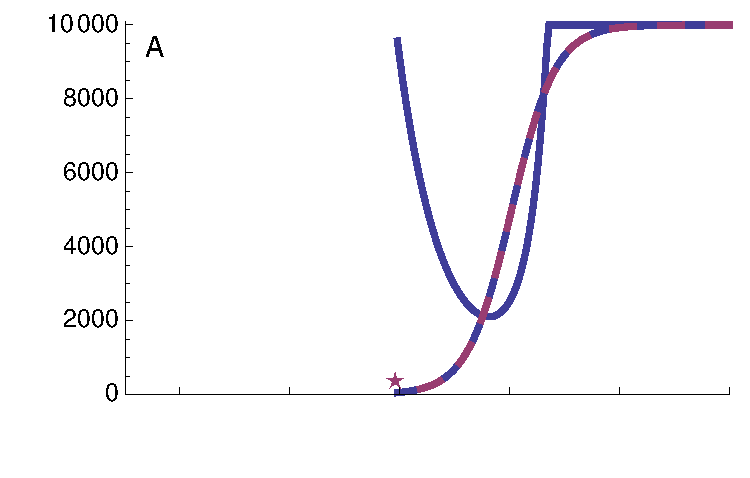
\includegraphics[width=0.49\linewidth]{dynamics_rescue_s0.2_k100_u0_m0.pdf}};
\node[below = -1cm of A1] (A2) {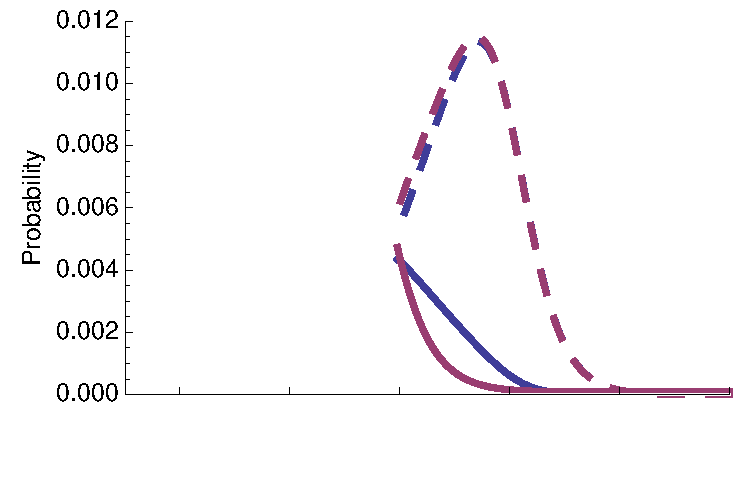
\includegraphics[width=0.49\linewidth]{coalescent_rescue_s0.2_k100_u0_m0.pdf}};
\node[right = 0cm of A1] (B1) {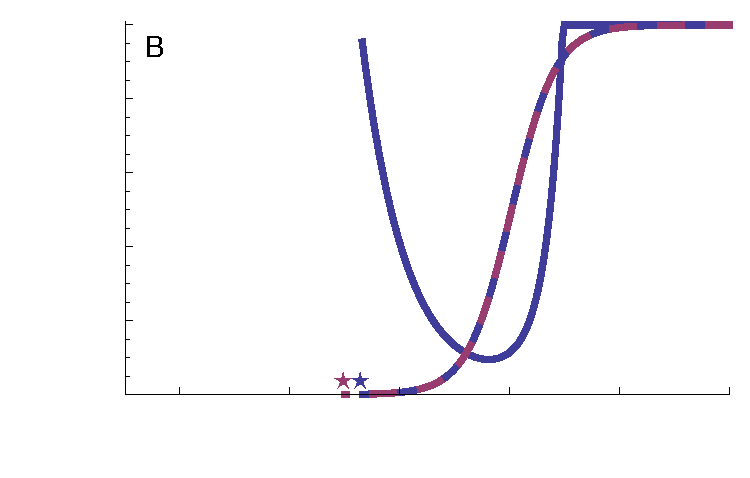
\includegraphics[width=0.49\linewidth]{dynamics_rescue_s0.2_k1_u0_m0.pdf}};
\node[right = 0cm of A2] (B2) {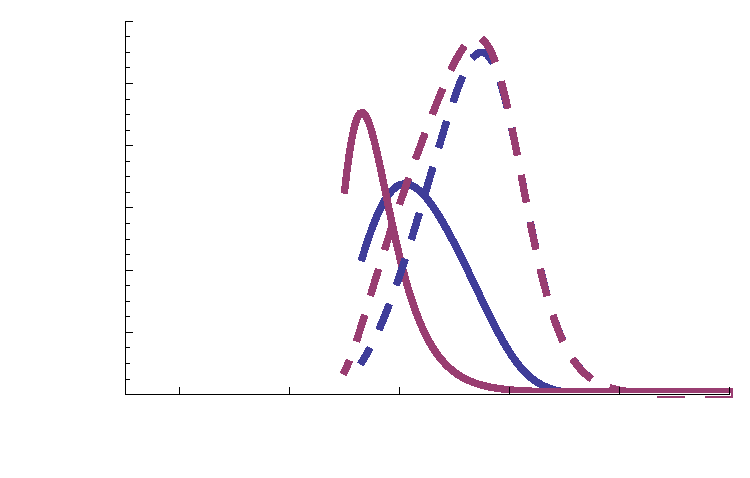
\includegraphics[width=0.49\linewidth]{coalescent_rescue_s0.2_k1_u0_m0.pdf}};
\node[below = 0cm of A2] (C1) {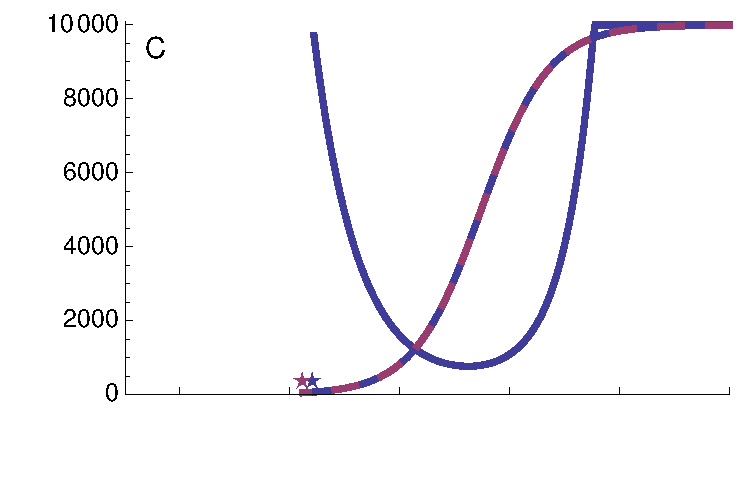
\includegraphics[width=0.49\linewidth]{dynamics_rescue_s0.13_k100_u0_m0.pdf}};
\node[below = -1cm of C1] (C2) {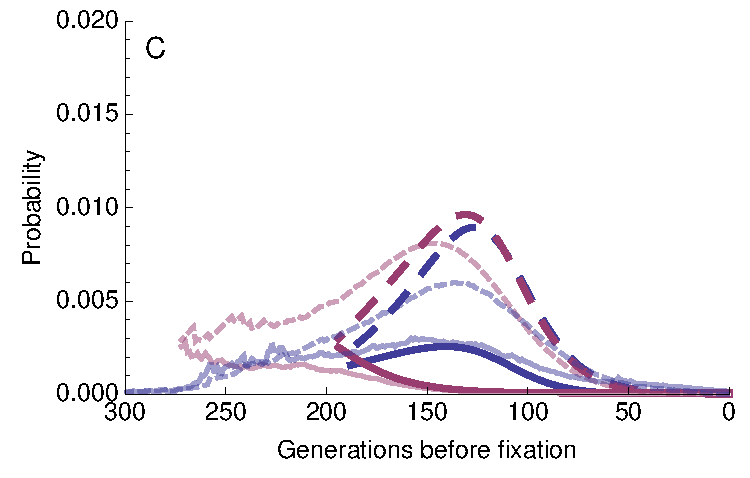
\includegraphics[width=0.49\linewidth]{coalescent_rescue_s0.13_k100_u0_m0.pdf}};
\node[right = 0cm of C1] (D1) {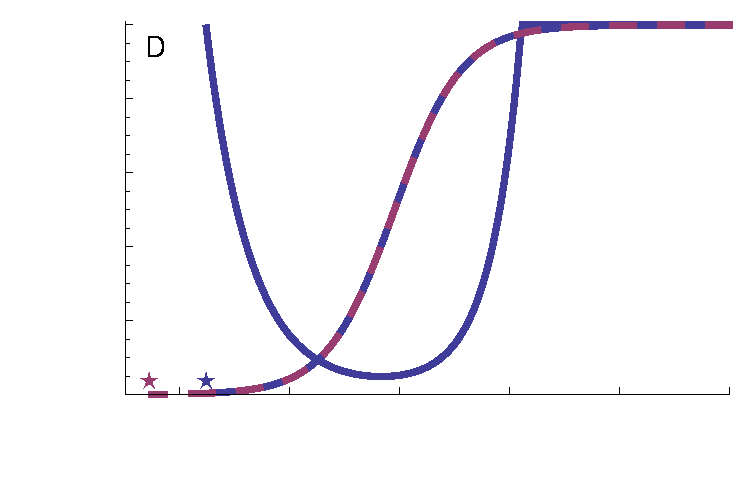
\includegraphics[width=0.49\linewidth]{dynamics_rescue_s0.13_k1_u0_m0.pdf}};
\node[right = 0cm of C2] (D2) {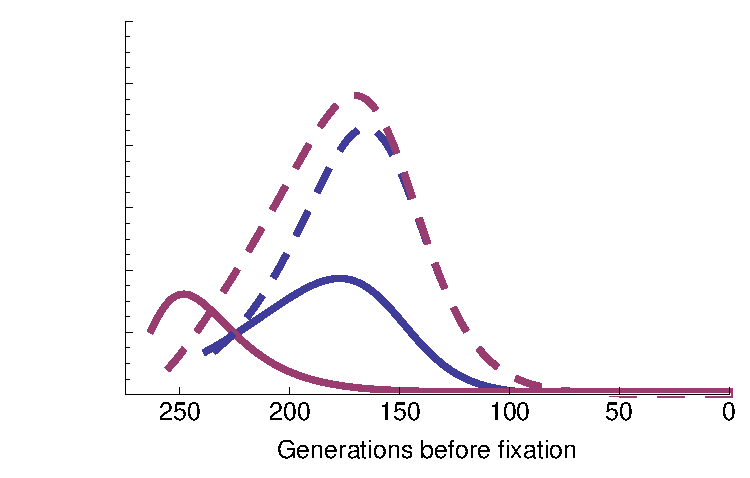
\includegraphics[width=0.49\linewidth]{coalescent_rescue_s0.13_k1_u0_m0.pdf}};
\node[right = 0.5 of A1, yshift = -2.5cm, rotate = 90, draw, rectangle, rounded corners, thick, fill=gray!50] (s) {\large$\bm{s=0.20}$};
\node[right = 0.5 of C1, yshift = -2.5cm, rotate = 90, draw, rectangle, rounded corners, thick, fill=gray!50] {\large$\bm{s=0.13}$};
\node[below = -0.6cm of A2, xshift = 20, draw, rectangle, rounded corners, thick, fill=gray!50] (k) {\large$\bm{\kappa=100}$};
\node[below = -0.6cm of B2, xshift = 20, draw, rectangle, rounded corners, thick, fill=gray!50] {\large$\bm{\kappa=1}$};
\node[right = 2cm of k, darkred, yshift = 0.25cm, draw, rectangle, rounded corners, thick, fill=darkred!25] (N) {\fontfamily{phv}\selectfont\textbf{constant $\bm{N}$}};
\node[below = 0cm of N, darkblue, draw, rectangle, rounded corners, thick, fill=darkblue!25] {\fontfamily{phv}\selectfont\textbf{evol.\ rescue}};
\node (pt) at ($(A1) + (-0.5cm,-0.5cm)$) {\footnotesize\fontfamily{phv}\selectfont sweep};
\draw (pt) -- ($(pt)+(1.5,-1/2)$);
\node (nt) at ($(A1) + (-1cm,1cm)$) {\footnotesize\fontfamily{phv}\selectfont bottleneck};
\draw (nt) -- ($(nt)+(1.4,-1/2)$);
\node (rec) at ($(A2) + (-1cm,1.5cm)$) {\footnotesize\fontfamily{phv}\selectfont recombination};
\draw (rec) -- ($(rec)+(1.4,-0.5)$);
\node (coal) at ($(A2) + (-1cm,-0.5cm)$) {\footnotesize\fontfamily{phv}\selectfont coalescence};
\draw (coal) -- ($(coal)+(1.4,-1/2)$);;
\end{tikzpicture}
\caption{
Timing of events in the history of a sample of size 2 at a linked neutral locus ($r=0.01$) during a selective sweep from standing genetic variation in evolutionary rescue (blue; $d=0.05$) or in a population of roughly constant size (red; $d=0$ such that $\mathbb{E}[N(t)]=N(0)$).
The top panel gives the approximate backwards-time dynamics (using Equation \ref{eq:ptnt}) for allele frequency $p'(\tau)$ (dashed; multiplied by $N(0)$ to be on the same scale as population size) and population size $N'(\tau)$ (solid; rescue only).
The stars are approximations of the fixation times $T$ (using Equation \ref{eq:ptnt}).
The bottom panel gives the resulting timings (Equation \ref{eq:Pikt}).
}%
\label{fig:rescueSGV_timing}
\end{figure}
%%%%%%%%%%%%%%%%%%%%%%%%%%%%%%%%%%%%%%%%%%%%%%%%

%%%%%%%%%%%%%%%%%%%%%%%%%%%%%%%%%%%%%%%%%%%%%%%%
\begin{figure}[htbp]
\centering
\begin{tikzpicture}
\node[] (A1) {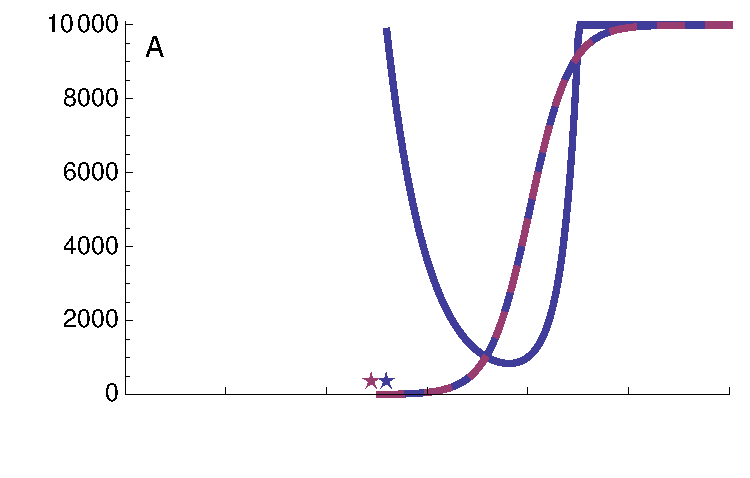
\includegraphics[width=0.49\linewidth]{dynamics_rescue_s0.2_k0_u0.0001_m0.pdf}};
\node[below = -1cm of A1] (A2) {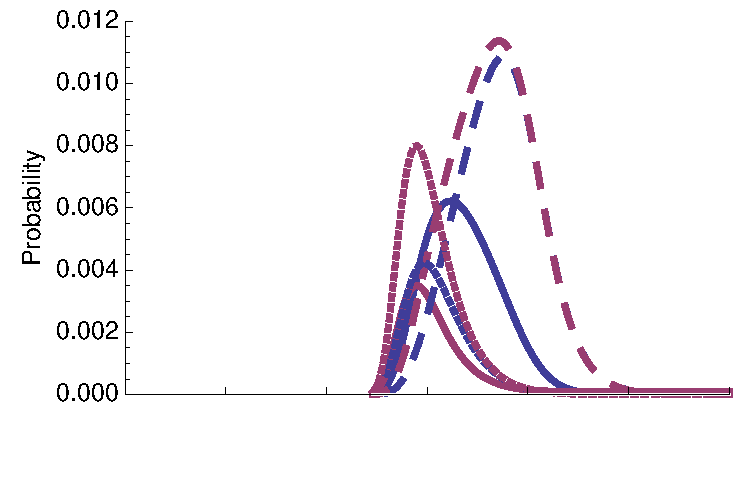
\includegraphics[width=0.49\linewidth]{coalescent_rescue_s0.2_k0_u0.0001_m0.pdf}};
\node[right = 0cm of A1] (B1) {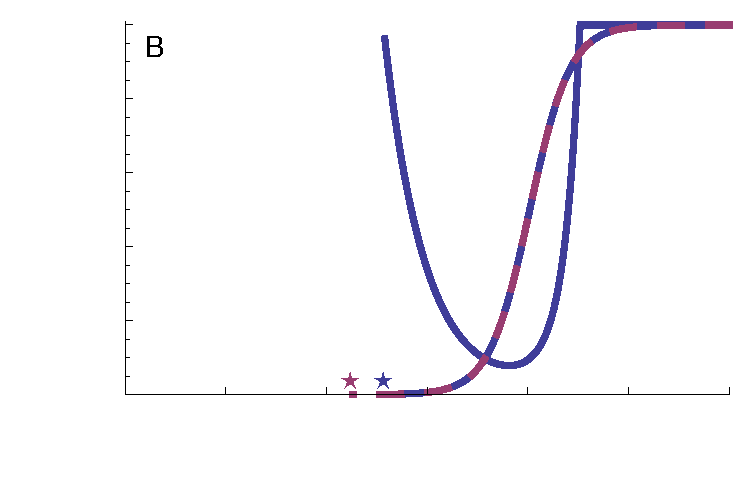
\includegraphics[width=0.49\linewidth]{dynamics_rescue_s0.2_k0_u0.00001_m0.pdf}};
\node[right = 0cm of A2] (B2) {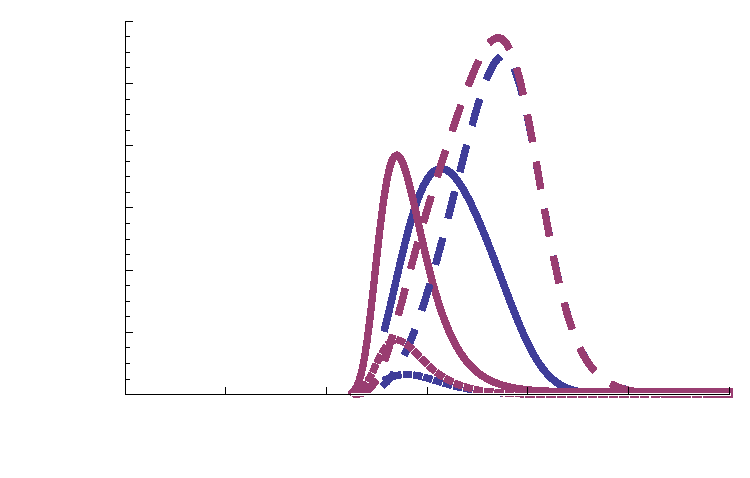
\includegraphics[width=0.49\linewidth]{coalescent_rescue_s0.2_k0_u0.00001_m0.pdf}};
\node[below = 0cm of A2] (C1) {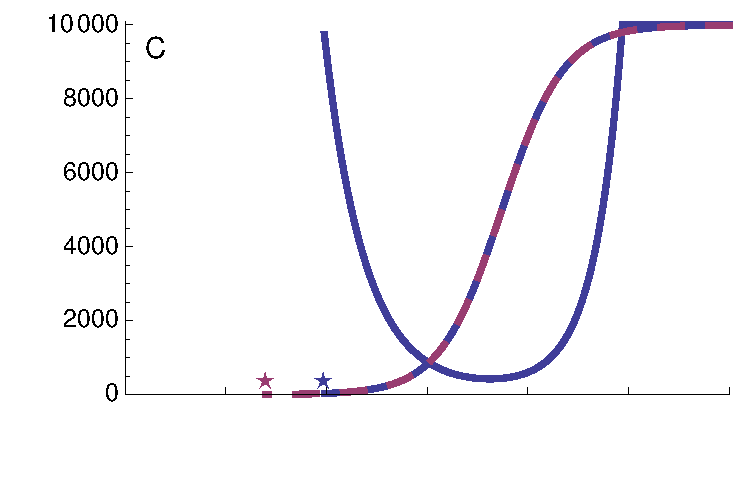
\includegraphics[width=0.49\linewidth]{dynamics_rescue_s0.13_k0_u0.0001_m0.pdf}};
\node[below = -1cm of C1] (C2) {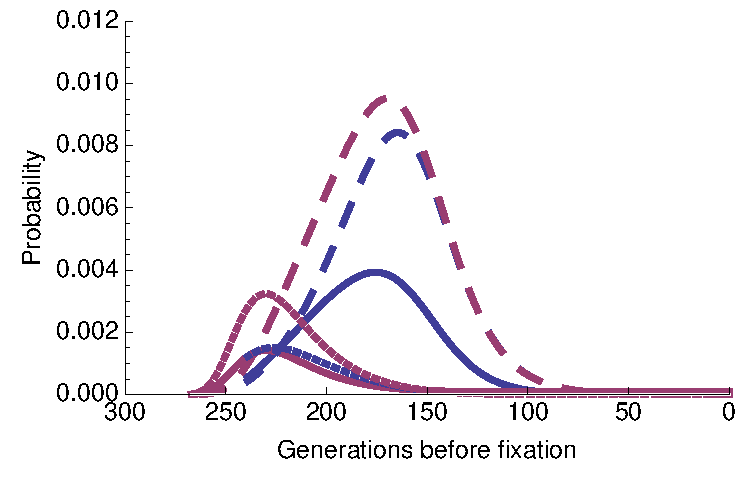
\includegraphics[width=0.49\linewidth]{coalescent_rescue_s0.13_k0_u0.0001_m0.pdf}};
\node[right = 0cm of C1] (D1) {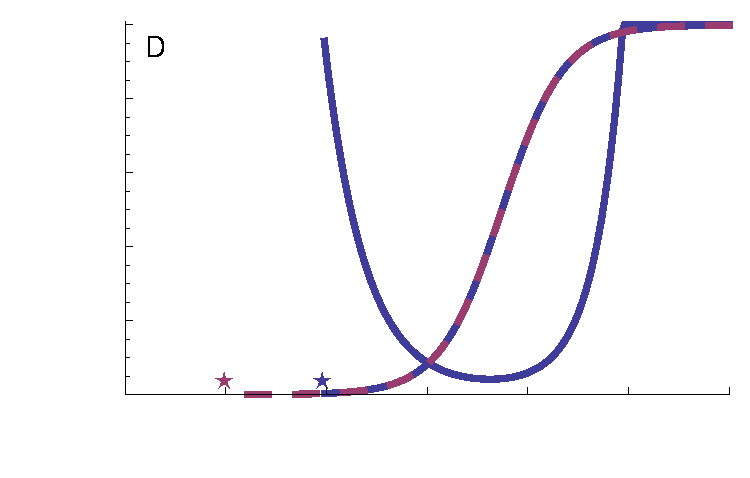
\includegraphics[width=0.49\linewidth]{dynamics_rescue_s0.13_k0_u0.00001_m0.pdf}};
\node[right = 0cm of C2] (D2) {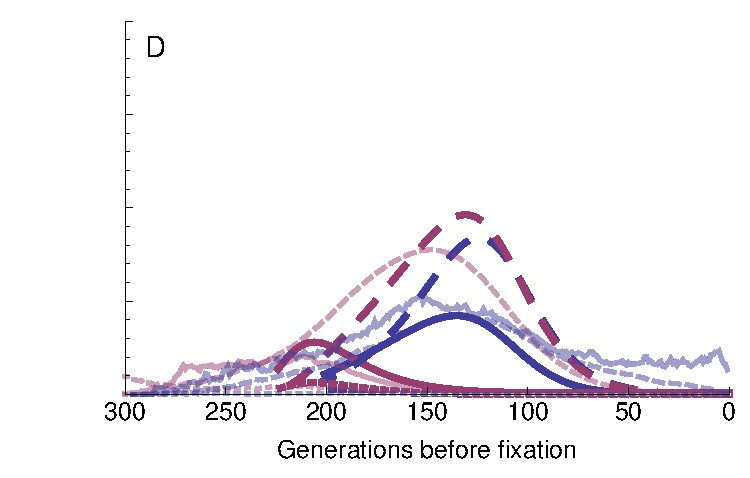
\includegraphics[width=0.49\linewidth]{coalescent_rescue_s0.13_k0_u0.00001_m0.pdf}};
\node[right = 0.5 of A1, yshift = -2.5cm, rotate = 90, draw, rectangle, rounded corners, thick, fill=gray!50] (s) {\large$\bm{s=0.20}$};
\node[right = 0.5 of C1, yshift = -2.5cm, rotate = 90, draw, rectangle, rounded corners, thick, fill=gray!50] {\large$\bm{s=0.13}$};
\node[below = -0.6cm of A2, xshift = 20, draw, rectangle, rounded corners, thick, fill=gray!50] (k) {\large$\bm{u=10^{-4}}$};
\node[below = -0.6cm of B2, xshift = 20, draw, rectangle, rounded corners, thick, fill=gray!50] {\large$\bm{u=10^{-5}}$};
\node[right = 2cm of k, darkred, yshift = 0.25cm, draw, rectangle, rounded corners, thick, fill=darkred!25] (N) {\fontfamily{phv}\selectfont\textbf{constant $\bm{N}$}};
\node[below = 0cm of N, darkblue, draw, rectangle, rounded corners, thick, fill=darkblue!25] {\fontfamily{phv}\selectfont\textbf{evol.\ rescue}};
\node (pt) at ($(A1) + (-0.5cm,-0.5cm)$) {\footnotesize\fontfamily{phv}\selectfont sweep};
\draw (pt) -- ($(pt)+(1.25,-1)$);
\node (nt) at ($(A1) + (-1cm,1cm)$) {\footnotesize\fontfamily{phv}\selectfont bottleneck};
\draw (nt) -- ($(nt)+(1.25,-1/2)$);
\node (rec) at ($(A2) + (-1cm,2cm)$) {\footnotesize\fontfamily{phv}\selectfont recombination};
\draw (rec) -- ($(rec)+(2,-1/2)$);
\node (mut) at ($(A2) + (-1cm,1cm)$) {\footnotesize\fontfamily{phv}\selectfont mutation};
\draw (mut) -- ($(mut)+(1.25,-1/2)$);
\node (coal) at ($(A2) + (3cm,0cm)$) {\footnotesize\fontfamily{phv}\selectfont coalescence};
\draw (coal) -- ($(coal)+(-1.5,-2/3)$);
\end{tikzpicture}
\caption{
Timing of events in the history of a sample of size 2 at a linked neutral locus ($r=0.01$) during a selective sweep from \textit{de novo} mutation in evolutionary rescue (blue; $d=0.05$) or in a population of roughly constant size (red; $d=0$).
See Figure \ref{fig:rescueSGV_timing} for details.
}%
\label{fig:rescueDNM_timing}
\end{figure}
%%%%%%%%%%%%%%%%%%%%%%%%%%%%%%%%%%%%%%%%%%%%%%%%

%%%%%%%%%%%%%%%%%%%%%%%%%%%%%%%%%%%%%%%%%%%%%%%%%%%
\subsection*{Genetic signatures at linked neutral loci}
\label{sec:rescue_signatures}

We now use the $P_i(k,\tau)$ to describe patterns of genetic variation at linked neutral loci in a random sample of chromosomes at (or not long after) the time of fixation.
Under rescue from standing genetic variance, we assume each of the $\kappa$ initial copies has independently arose via mutation in the recent past, which assumes the allele was sufficiently deleterious before the environmental change \citep[c.f.,][]{prezeworski2005signature}.
We neglect the migration case as this requires a number of assumptions about the history of the metapopulation, e.g., how and when the sweeps occurred in the neighbouring patches, historical migration rates, etc.

%%%%%%%%%%%%%%%%%%%%%%%%%%%%%%%%%%%%%%%%%%%%%%%%%%%
\subsubsection*{Genetic diversity}
\label{sec:rescue_heterozygosity}

One classic pattern of genetic variation produced by a selective sweep is a dip in genetic diversity around the selected site \citep{smith1974hitch,kaplan1989hitchhiking}. 
Here we consider the average number of nucleotide differences between two randomly sampled sequences, $\pi$ \citep{tajima1983evolutionary}, focusing on sequences of length 1 (i.e., heterozygosity).

We first consider our expectation for $\pi$ at a site that is far enough away from the selected site to be unaffected by the sweep; this provides us with an expectation for the genome-wide average, which is determined by the mutation rate at neutral loci and the population bottleneck.
In particular, our expectation for $\pi$ at such a site in a population of constant effective size, $N_e$, is simply $\theta = 4 N_e U$ \citep{watterson1975number}, with $U$ the per base per generation mutation rate at neutral loci.
Ignoring neutral mutation input during the bottleneck, the $\pi$ at a sufficiently loosely linked site is this neutral expectation times the probability a sample of size two does not coalesce during the period of interest (in our case, from the time we take the sample at the time of fixation, $t=T$, until the time of environmental change, $t=0$).
This is (c.f., equation 4 in \citealp{slatkin1991pairwise} and equation 7 in \citealp{griffiths1994sampling})
\begin{equation}\label{eq:EH_rescue_loose}
\mathbb{E}[\pi | \mathrm{unlinked}]\approx \theta \exp \left( - \int_0^T p_{\mathrm{coal}}(2,\tau) \mathrm{d}\tau \right) = \theta \exp \left( - \int_0^T \frac{1}{2N_e'(\tau)} \mathrm{d}\tau \right). 
\end{equation}

We next consider sites that are more closely linked to the selected locus, and are thus directly affected by the selective sweep.
To keep the analysis simple, we assume that if one of the sampled alleles recombines or mutates off the beneficial background before the two samples coalesce then it is as if both samples were on the ancestral background from the start and therefore coalesce with each other as if they were at an unlinked locus (Equation \ref{eq:EH_rescue_loose}).
This assumption will be appropriate with large recombination and mutation rates, where both samples will quickly recombine or mutate off the sweep, and with small recombination and mutation rates, where coalescence will typically occur first.
At moderate recombination and mutation rates we will tend to underestimate diversity as the second recombination or mutation event will then take place further back in the past, restricting the time over which the samples can coalesce.
Finally, there is also the possibility of no events occurring in the history of the sample during the sweep; if the sweep arose from mutation (or migration) or from a single copy of the beneficial allele ($\kappa=1$) then the sample must coalesce, otherwise (i.e., if we start with more than one beneficial copy, $\kappa>1$), under our assumption that each copy of the beneficial allele among the standing variance has a unique mutational origin, the samples are independent draws from a neutral population.
Ignoring neutral mutations during the sweep, a simple approximation for $\pi$ at any location in the genome is then
\begin{equation}\label{eq:EH_rescue}
\begin{aligned}
\mathbb{E}[\pi ] \approx \mathbb{E}[\pi | \mathrm{unlinked}] \left[ P_\mathrm{off}(2,T) + P_\emptyset(2,T) \delta_{\kappa>1} \right],
\end{aligned}
\end{equation}
where $P_\mathrm{off}(k,T) = \int_0^T [P_\mathrm{rec}(k,\tau) + P_\mathrm{mut}(k,\tau) ] \mathrm{d}\tau$ is the probability of recombination or mutation before coalescence during the sweep, $P_\emptyset(k, T) = \exp \left( -\sum_{j} \int_{0}^T p_{j}(k,\tau) \mathrm{d}\tau \right)$ is the probability that no events have occurred in the history of the sample during the sweep ($j\in\{\mathrm{rec},\mathrm{mut},\mathrm{coal}\}$), and $\delta_{\kappa>1}$ is 1 if the sweep arose from more than one copy of the beneficial allele ($\kappa>1$) and 0 otherwise.

Figures \ref{fig:rescueSGV_heterozygosity}-\ref{fig:rescueDNM_heterozygosity} compare our predictions of $\pi$ after evolutionary rescue against both simulations and the constant population size scenario ($d=0$). 
While our predictions qualitatively match simulations, the tendency of our deterministic approximations to overestimate population size when the probability of rescue is small (Figures \ref{fig:rescueSGV_dynamics} and \ref{fig:rescueDNM_dynamics}) causes us to overestimate diversity in these cases.
To correct for this, in Figures \ref{fig:rescueSGV_heterozygosity_empirical}-\ref{fig:rescueDNM_heterozygosity_empirical} we replace our prediction for $\mathbb{E}[\pi | \mathrm{unlinked}]$ (Equation \ref{eq:EH_rescue_loose}) in the rescue scenario with the observed mean diversity level (as a technical aside, because we only simulate a 40cM chromosome, much of which is affected by the sweep, we do not use sites within 5cM of the selected locus in our average; including these sites would have very little effect in larger genomes).
A very similar result was achieved by converting the observed population sizes to effective population sizes and computing the sum in Equation \ref{eq:EH_rescue_loose} (results not shown). 
Using the observed mean diversity level is justified by the fact that genome-wide diversity can be measured directly from data and is highly variable across populations \citep{tajima1983evolutionary}.
In fact, unless the population was sampled both before and after the selective sweep (or we have good estimates of its mutation rate and long-term effective population size), the amount of background pairwise diversity tells us very little about recent population size changes and all the information is contained in relative diversity (the diversity in a window divided by genome-wide diversity).
Figures \ref{fig:rescueSGV_heterozygosity_relative}-\ref{fig:rescueDNM_heterozygosity_relative} show that our predictions of relative diversity ($\mathbb{E}[\pi]/\mathbb{E}[\pi|\mathrm{unlinked}$) closely match that observed in simulations.

Figures \ref{fig:rescueSGV_heterozygosity_empirical}-\ref{fig:rescueDNM_heterozygosity_empirical} and \ref{fig:rescueSGV_heterozygosity_relative}-\ref{fig:rescueDNM_heterozygosity_relative} show that evolutionary rescue has three main effects relative to the constant population case:
1) rescue can greatly reduce genome-wide diversity under sufficiently weak selection, where bottlenecks are long and deep (by increasing $T$ and decreasing $N_e(\tau)$; Equation \ref{eq:EH_rescue_loose}),
2) rescue tends to deepen dips in diversity when soft sweeps are possible, i.e., it hardens soft sweeps (by decreasing $P_\mathrm{off}(2,T)$ at the selected site, $r=0$; Equation \ref{eq:EH_rescue}), and
3) rescue generally produces wider dips in diversity due to excess coalescence during the sweep (by decreasing $P_\mathrm{off}(2,T)$ at a given $r>0$; Equation \ref{eq:EH_rescue}).

%%%%%%%%%%%%%%%%%%%%%%%%%%%%%%%%%%%%%%%%%%%%%%%
\begin{figure}[htb]
\centering
\begin{tikzpicture}
\node[] (A) {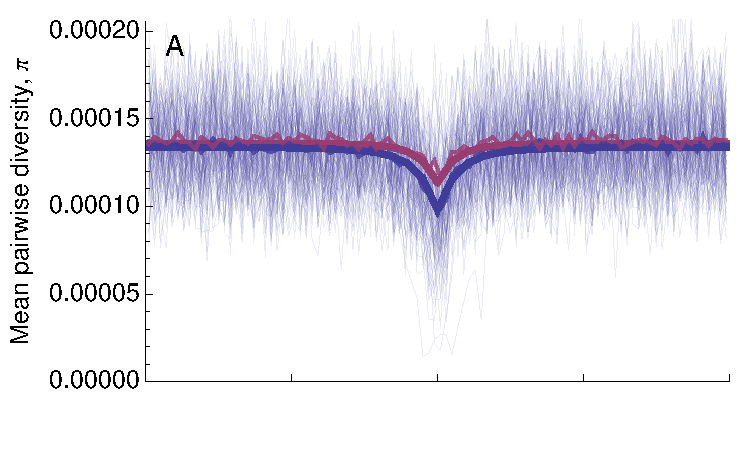
\includegraphics[width=0.49\linewidth]{EH_rescue_s0.2_k100_u0_m0_empirical.pdf}};
\node[right = 0 of A] (B) {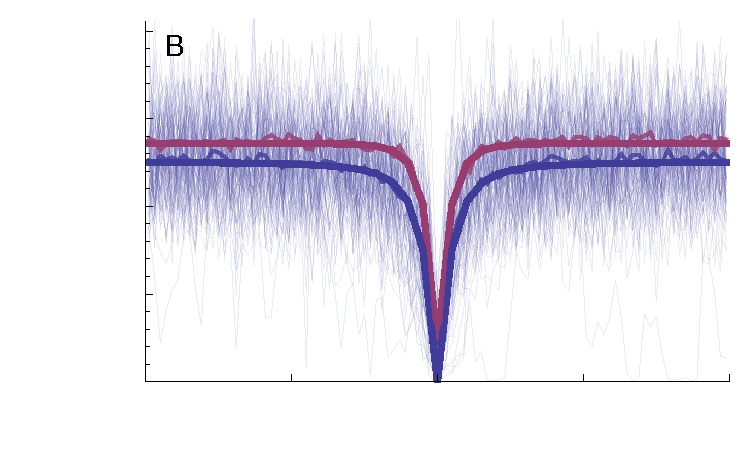
\includegraphics[width=0.49\linewidth]{EH_rescue_s0.2_k1_u0_m0_empirical.pdf}};
\node[below = 0 of A] (C) {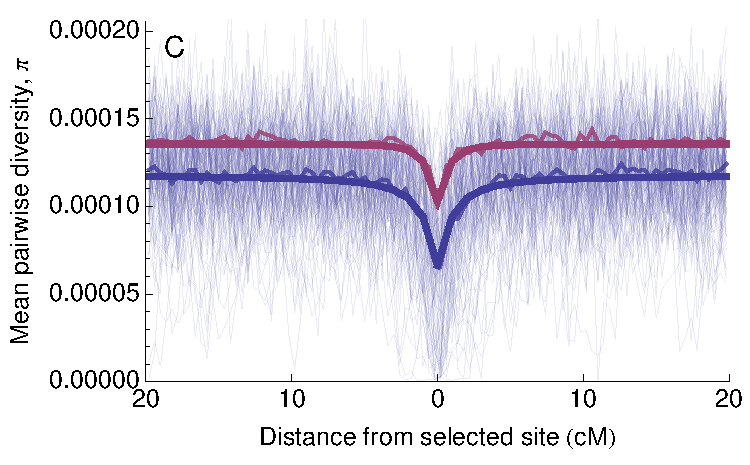
\includegraphics[width=0.49\linewidth]{EH_rescue_s0.13_k100_u0_m0_empirical.pdf}};
\node[right = 0 of C] (D) {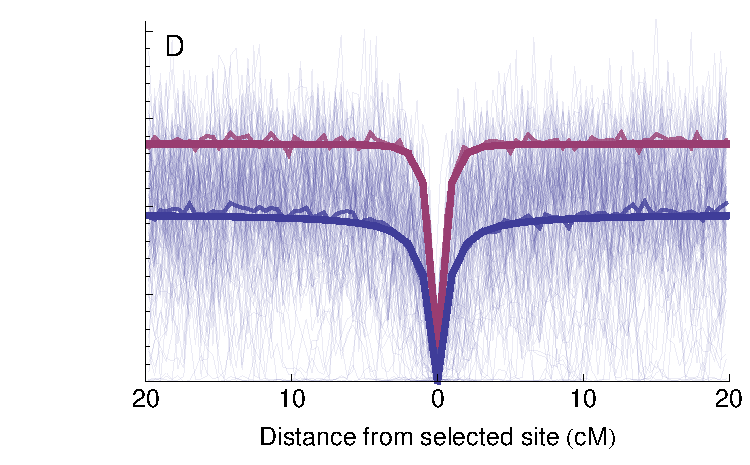
\includegraphics[width=0.49\linewidth]{EH_rescue_s0.13_k1_u0_m0_empirical.pdf}};
\node[right = 0 of A, xshift = 0.6cm, yshift = -0.5cm, draw, rectangle, rounded corners, thick, fill=gray!50, rotate = 90] (s) {\large$\bm{s=0.20}$};
\node[right = 0 of C,  xshift = 0.6cm, yshift = -0.5cm, draw, rectangle, rounded corners, thick, fill=gray!50, rotate = 90] {\large$\bm{s=0.13}$};
\node[below = -2/3 of A, xshift = 20, draw, rectangle, rounded corners, thick, fill=gray!50] (k) {\large$\bm{\kappa=100}$};
\node[below = -2/3 of B, xshift = 20, draw, rectangle, rounded corners, thick, fill=gray!50] {\large$\bm{\kappa=1}$};
\node[right = 2cm of k, darkred, yshift = 0.25cm, draw, rectangle, rounded corners, thick, fill=darkred!25] (N) {\fontfamily{phv}\selectfont \textbf{constant $\bm{N}$}};
\node[below = 0 of N, darkblue, draw, rectangle, rounded corners, thick, fill=darkblue!25] {\fontfamily{phv}\selectfont \textbf{evol.\ rescue}};
\end{tikzpicture}
\caption{
Mean pairwise diversity, $\pi$, after a selective sweep from standing genetic variation during evolutionary rescue (blue; $d=0.05$) or in a population of roughly constant size (red; $d=0$ such that $\mathbb{E}[N(t)]=N(0)$).
The thick curves are Equation \ref{eq:EH_rescue}; for rescue (blue) we use the observed mean diversity as $\theta$.
The thinnest curves are 100 replicate simulations (rescue only for clarity) and the slightly thicker curves are simulation means (often obscured by prediction).
Parameters: $N(0)=10^4$.
}%
\label{fig:rescueSGV_heterozygosity_empirical}
\end{figure}
%%%%%%%%%%%%%%%%%%%%%%%%%%%%%%%%%%%%%%%%%%%%%%%

%%%%%%%%%%%%%%%%%%%%%%%%%%%%%%%%%%%%%%%%%%%%%%%
\begin{figure}[htb]
\centering
\begin{tikzpicture}
\node[] (A) {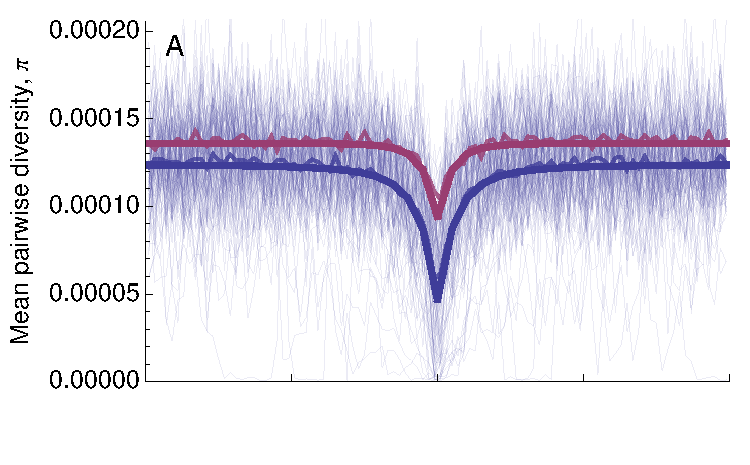
\includegraphics[width=0.49\linewidth]{EH_rescue_s0.2_k0_u0.0001_m0_empirical.pdf}};
\node[right =0 of A] (B) {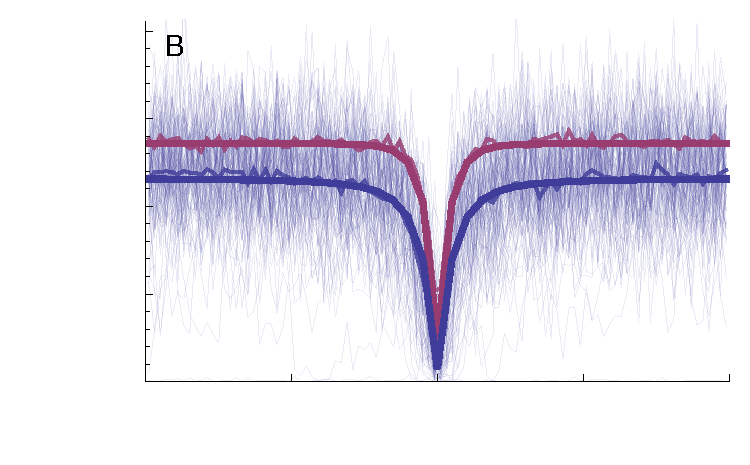
\includegraphics[width=0.49\linewidth]{EH_rescue_s0.2_k0_u0.00001_m0_empirical.pdf}};
\node[below =0 of A] (C) {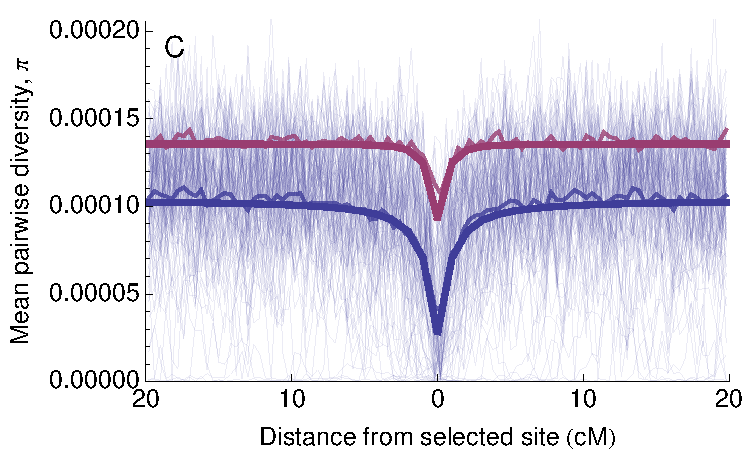
\includegraphics[width=0.49\linewidth]{EH_rescue_s0.13_k0_u0.0001_m0_empirical.pdf}};
\node[right =0 of C] (D) {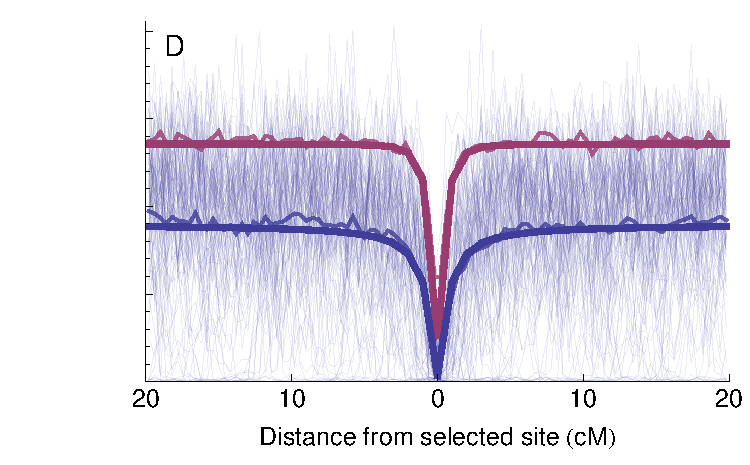
\includegraphics[width=0.49\linewidth]{EH_rescue_s0.13_k0_u0.00001_m0_empirical.pdf}};
\node[right = 0 of A, xshift = 0.6cm, yshift = -0.5cm, draw, rectangle, rounded corners, thick, fill=gray!50, rotate = 90] (s) {\large$\bm{s=0.20}$};
\node[right = 0 of C,  xshift = 0.6cm, yshift = -0.5cm, draw, rectangle, rounded corners, thick, fill=gray!50, rotate = 90] {\large$\bm{s=0.13}$};
\node[below = -2/3 of A, xshift = 20, draw, rectangle, rounded corners, thick, fill=gray!50] (k) {\large$\bm{u=10^{-4}}$};
\node[below = -2/3 of B, xshift = 20, draw, rectangle, rounded corners, thick, fill=gray!50] {\large$\bm{u=10^{-5}}$};
\node[right = 2cm of k, darkred, yshift = 0.25cm, draw, rectangle, rounded corners, thick, fill=darkred!25] (N) {\fontfamily{phv}\selectfont \textbf{constant $\bm{N}$}};
\node[below = 0 of N, darkblue, draw, rectangle, rounded corners, thick, fill=darkblue!25] {\fontfamily{phv}\selectfont \textbf{evol.\ rescue}};
\end{tikzpicture}
\caption{
Mean pairwise diversity, $\pi$, after a selective sweep from \textit{de novo} mutation during evolutionary rescue (blue; $d=0.05$) or in a population of roughly constant size (red; $d=0$).
See Figure \ref{fig:rescueSGV_heterozygosity_empirical} for details.
}%
\label{fig:rescueDNM_heterozygosity_empirical}
\end{figure}
%%%%%%%%%%%%%%%%%%%%%%%%%%%%%%%%%%%%%%%%%%%%%%%

%%%%%%%%%%%%%%%%%%%%%%%%%%%%%%%%%%%%%%%%%%%%%%%%%%%
\subsubsection*{Tajima's \textit{D}}
\label{sec:tajimasD}

Finally, we consider Tajima's $D$ statistic \citep{tajima1989statistical}, which measures the relative excess (positive $D$) or deficiency (negative $D$) of intermediate frequency polymorphisms, relative to the standard neutral model (i.e., constant population size, neutral evolution). 
Quantitative predictions of Tajima's $D$ require one to consider samples of size greater than 2, which quickly becomes complicated with selection and complex demography.
Instead, here we discuss the expected qualitative patterns, based on intuition from the analysis presented above, and compare these to simulation results.

First, hard selective sweeps tend to produce star-like gene genealogies, with most samples coalescing near the beginning of the sweep and recombination allowing a few samples to coalesce much further back in time \citep{kaplan1989hitchhiking}.
Hard sweeps therefore produce an excess of low frequency polymorphisms \citep[][p.\ 120]{wakeley2009coalescent}, leading to negative $D$ \citep{braverman1995hitchhiking}.
The larger the selection coefficient the more star-like the genealogy (less time for coalescence or recombination during the sweep), and thus the more negative $D$ when conditioned on a hard sweep.
However, with sufficient standing genetic variation or rates of recurrent mutation or migration, larger selection coefficients will tend to cause softer selective sweeps (Figures \ref{fig:PsoftSGV}, \ref{fig:PsoftDNM}, and \ref{fig:PsoftMIG}).
Soft selective sweeps allow samples to coalesce further back in time, before the start of the sweep, even at the selected site.
Such sweeps therefore tend to have less effect on neutral genealogies and hence on $D$, although sufficiently soft sweeps can actually cause positive $D$, by allowing intermediate-sized groups of samples to descend from different ancestors containing the beneficial allele \citep{pennings2006soft}.

As linkage to the selected site decreases so too does this skew in genealogies.
In the case of a constant population size, $D$ should asymptote to the neutral expectation of zero.
In the case of rescue, however, the bottleneck will cause an excess of intermediate frequency polymorphisms \citep[][p.\ 120]{wakeley2009coalescent}, and therefore $D$ should asymptote at some positive value (more positive with more severe bottlenecks).
 
These patterns are borne out in simulations (Figures \ref{fig:rescueSGV_tajimasD}-\ref{fig:rescueDNM_tajimasD}), where we see that rescue consistently causes positive background $D$.
When sweeps are guaranteed to be hard ($\kappa=1$), $D$ around the selected site is similarly negative in both rescue and under a constant population size.
When there is some possibility for a soft sweep (all cases but $\kappa=1$), rescue tends to harden the sweep (by reducing probabilities of establishment, increasing coalescence, and reducing mutational input) and thus produce lower values of $D$ at the selected site.
Together these patterns cause rescue to stretch out or even invert the pattern of $D$ observed in populations of constant size: under rescue, $D$ tends to be greater away from the selected site and lower at the selected site.

%%%%%%%%%%%%%%%%%%%%%%%%%%%%%%%%%%%%%%%%%%%%%%%
\begin{figure}[htb]
\centering
\begin{tikzpicture}
\node[] (A) {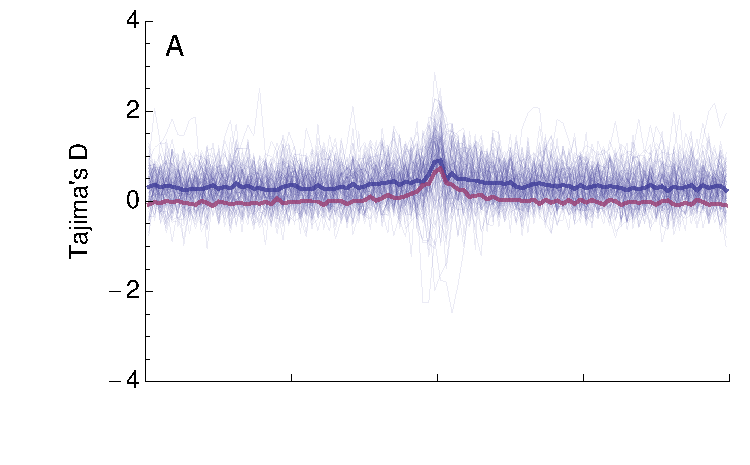
\includegraphics[width=0.49\linewidth]{TajimasD_rescue_s0.2_k100_u0_m0.pdf}};
\node[right =0 of A] (B) {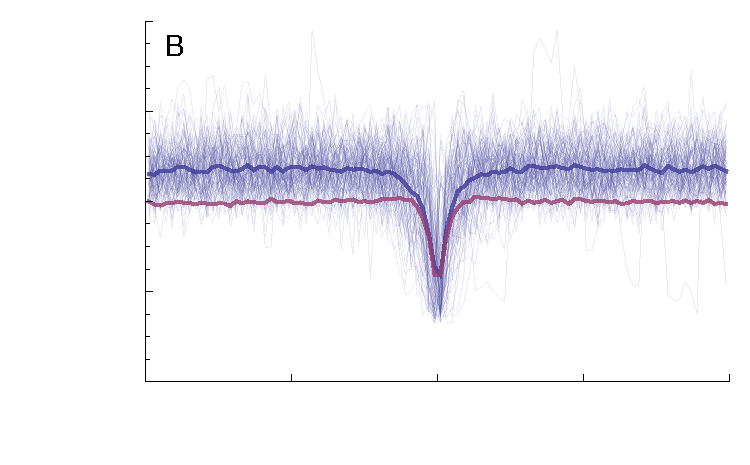
\includegraphics[width=0.49\linewidth]{TajimasD_rescue_s0.2_k1_u0_m0.pdf}};
\node[below =0 of A] (C) {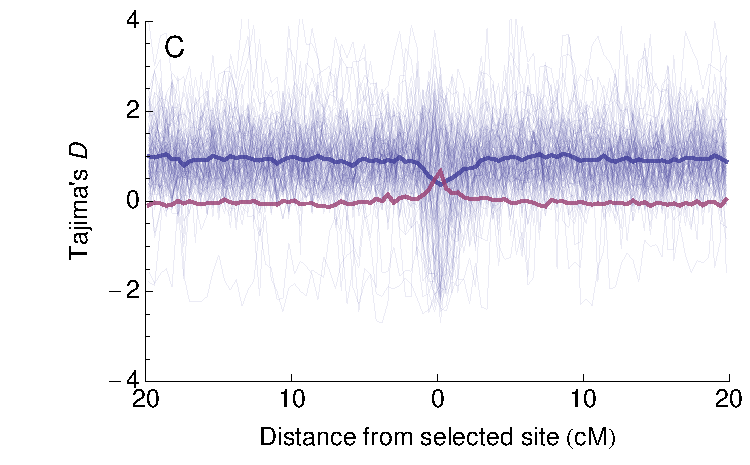
\includegraphics[width=0.49\linewidth]{TajimasD_rescue_s0.13_k100_u0_m0.pdf}};
\node[right =0 of C] (D) {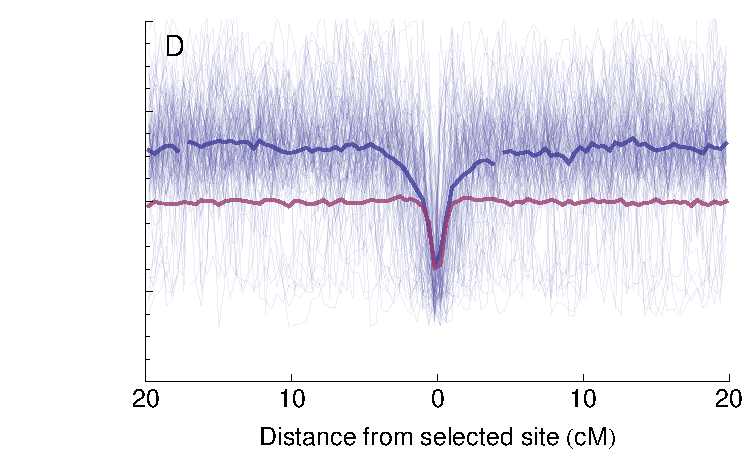
\includegraphics[width=0.49\linewidth]{TajimasD_rescue_s0.13_k1_u0_m0.pdf}};
\node[right = 0 of A, xshift = 0.6cm, yshift = -0.5cm, draw, rectangle, rounded corners, thick, fill=gray!50, rotate = 90] (s) {\large$\bm{s=0.20}$};
\node[right = 0 of C,  xshift = 0.6cm, yshift = -0.5cm, draw, rectangle, rounded corners, thick, fill=gray!50, rotate = 90] {\large$\bm{s=0.13}$};
\node[below = -2/3 of A, xshift = 20, draw, rectangle, rounded corners, thick, fill=gray!50] (k) {\large$\bm{\kappa=100}$};
\node[below = -2/3 of B, xshift = 20, draw, rectangle, rounded corners, thick, fill=gray!50] {\large$\bm{\kappa=1}$};
\node[right = 2cm of k, darkred, yshift = 0.25cm, draw, rectangle, rounded corners, thick, fill=darkred!25] (N) {\fontfamily{phv}\selectfont \textbf{constant $\bm{N}$}};
\node[below = 0 of N, darkblue, draw, rectangle, rounded corners, thick, fill=darkblue!25] {\fontfamily{phv}\selectfont \textbf{evol.\ rescue}};
\end{tikzpicture}
\caption{
Tajima's $D$ after a selective sweep from standing genetic variation during evolutionary rescue (blue; $d=0.05$) or in a population of roughly constant size (red; $d=0$ such that $\mathbb{E}[N(t)]=N(0)$).
Thin curves show 100 replicate simulations (rescue only for clarity) and thicker curves show simulation means.
Parameters: $N(0)=10^4$.
}%
\label{fig:rescueSGV_tajimasD}
\end{figure}
%%%%%%%%%%%%%%%%%%%%%%%%%%%%%%%%%%%%%%%%%%%%%%%

%%%%%%%%%%%%%%%%%%%%%%%%%%%%%%%%%%%%%%%%%%%%%%%
\begin{figure}[htb]
\centering
\begin{tikzpicture}
\node[] (A) {\includegraphics[width=0.49\linewidth]{TajimasD_rescue_s0.2_k0_u0.0001_m0.pdf}};
\node[right =0 of A] (B) {\includegraphics[width=0.49\linewidth]{TajimasD_rescue_s0.2_k0_u0.00001_m0.pdf}};
\node[below =0 of A] (C) {\includegraphics[width=0.49\linewidth]{TajimasD_rescue_s0.13_k0_u0.0001_m0.pdf}};
\node[right =0 of C] (D) {\includegraphics[width=0.49\linewidth]{TajimasD_rescue_s0.13_k0_u0.00001_m0.pdf}};
\node[right = 0 of A, xshift = 0.6cm, yshift = -0.5cm, draw, rectangle, rounded corners, thick, fill=gray!50, rotate = 90] (s) {\large$\bm{s=0.20}$};
\node[right = 0 of C,  xshift = 0.6cm, yshift = -0.5cm, draw, rectangle, rounded corners, thick, fill=gray!50, rotate = 90] {\large$\bm{s=0.13}$};
\node[below = -2/3 of A, xshift = 20, draw, rectangle, rounded corners, thick, fill=gray!50] (k) {\large$\bm{u=10^{-4}}$};
\node[below = -2/3 of B, xshift = 20, draw, rectangle, rounded corners, thick, fill=gray!50] {\large$\bm{u=10^{-5}}$};
\node[right = 2cm of k, darkred, yshift = 0.25cm, draw, rectangle, rounded corners, thick, fill=darkred!25] (N) {\fontfamily{phv}\selectfont \textbf{constant $\bm{N}$}};
\node[below = 0 of N, darkblue, draw, rectangle, rounded corners, thick, fill=darkblue!25] {\fontfamily{phv}\selectfont \textbf{evol.\ rescue}};
\end{tikzpicture}
\caption{
Tajima's $D$ after a selective sweep from \textit{de novo} mutation during evolutionary rescue (blue; $d=0.05$) or in a population of roughly constant size (red; $d=0$ such that $\mathbb{E}[N(t)]=N(0)$).
See Figure \ref{fig:rescueSGV_tajimasD} for details.
}%
\label{fig:rescueDNM_tajimasD}
\end{figure}
%%%%%%%%%%%%%%%%%%%%%%%%%%%%%%%%%%%%%%%%%%%%%%%

%%%%%%%%%%%%%%%%%%%%%%%%%%%%%%%%%%%%%%%%%%%%%%%%%%%
\section*{Discussion}
\label{sec:discussion}

%%major findings
Here we have explored genetic signatures of evolutionary rescue by a selective sweep. 
By allowing demography to depend on the absolute fitness of the genotypes that comprise the population we explicitly invoke a feedback between demography and evolution.
This feedback restricts the range of dynamics, and thus the signatures, that one should expect to observe.
We find that, because the probability of establishment for an allele with a given selective advantage is reduced in declining populations \citep[Equation \ref{eq:pest}; see also][]{otto1997probability}, selective sweeps causing rescue are expected to be harder than those in populations of constant size when sweeps arise from standing genetic variance or recurrent mutation (Figures \ref{fig:PsoftSGV} and \ref{fig:PsoftDNM}; consistent with \citealp{wilson2014soft} and \citealp{wilson2017soft}).
Further from the selected locus, the demographic bottleneck experienced during rescue increases rates of coalescence relative to mutation and recombination (Figures \ref{fig:rescueSGV_timing}-\ref{fig:rescueDNM_timing}), creating wider dips in diversity and lower diversity genome-wide (Figures \ref{fig:rescueSGV_heterozygosity_empirical}-\ref{fig:rescueDNM_heterozygosity_empirical}; consistent with \citealp{innan2004pattern}). 
Tajima's $D$ captures both the hardening of the sweep and the bottleneck, causing $D$ to generally reach both higher and lower values under rescue (Figures \ref{fig:rescueSGV_tajimasD}-\ref{fig:rescueDNM_tajimasD}).
These differences between evolutionary rescue and standard sweeps all become larger under weaker selection (i.e., when the heterozygote has a smaller growth rate, $s/2-d\ll1$) as the slower sweeps that result imply deeper, longer bottlenecks during rescue.
In contrast to standing variance or mutation, when sweeps arise from a constant rate of migration demography has no affect on the number of beneficial alleles that establish \citep[as briefly noted by][]{pennings2006soft2} and thus rescue has no affect on the hardness of the sweep (Figure \ref{fig:PsoftMIG}). 
Further, because the rates of coalescence and migration are both inversely proportional to the number of beneficial alleles $N(t)p(t)$ at the selected site (Equation \ref{eq:coal_rates}, Figure \ref{fig:rescueMIG_timing}), the distribution of the number and frequency of migrant haplotypes spanning the selected site is given by Ewens' sampling formula \citep{ewens1972sampling}, with mutation replaced by migration \citep{pennings2006soft2}.
As we move away from the selected site recombination breaks apart these migrant haplotypes, leading to patterns of nucleotide diversity that depend on the migration rate and history of the two populations.
If the migration rate is low we should expect an excess of migrant haplotypes at the site of the selective introgression and, if the divergence between the migrant and focal population is high, the so-called ``volcano" pattern of diversity \citep{setter2019volcanofinder}, where diversity is maximized at an intermediate distance from the selected site due to a more balanced presence of both migrant and non-migrant alleles.

%%unanswered questions
Evolutionary rescue has been explored theoretically \citep[e.g.,][]{gomulkiewicz1995does,uecker2016role,anciaux2018evolutionary} and observed repeatedly in both experiments \citep[e.g.,][]{bell2009evolutionary,lindsey2013evolutionary,ramsayer2013evolutionary} and in host-pathogen systems in nature \citep[e.,g.,][]{wei1995viral,feder2016more}.
More recently, a number of studies have used genetic data to suggest that evolutionary rescue has occurred in the wild, including crickets becoming song-less to avoid parasitoid flies (\citealp{pascoal2018silent}, reviewed in \citealp{mcdermott2019news}), killifish deleting receptors to tolerate pollution \citep{oziolor2019adaptive}, hares moulting brown instead of white to avoid predation in snowless winters \citep{jones2018adaptive}, bats altering hibernation to survive white-nose syndrome \citep{gignoux2018genomic}, and tall waterhemp evolving herbicide resistance \citep{kreiner2019multiple}.
In nearly all of these cases there is strong evidence of a recent selective sweep by a very beneficial allele.
Genetic evidence for a demographic bottleneck, on the other hand, is generally lacking, although genome-wide reductions in nucleotide diversity and increases in Tajima's $D$, relative to non-stressed populations, are sometimes detected \citep{oziolor2019adaptive}.
This begs the question of whether one can infer evolutionary rescue from genetic data alone, which would greatly help in assessing the relevance of rescue in nature.
Strong support for rescue would come from the coincident timing of a sweep and bottleneck, which is difficult given the imprecise time estimates from a genetic sample collected from a single time point.  
Sampling before and after the potential rescue event would therefore be highly advantageous in determining co-occurrence.
However, it should be noted that even if the sweep and bottleneck appear to have co-occurred, this correlation in timing does not imply it was caused by a feedback between demography and evolution. 
It is, of course, difficult to say in any case -- without observing replicate populations go extinct or performing experiments -- whether extinction would have occurred (or will occur) without adaptive evolution, as required by the strict definition of evolutionary rescue.
We therefore need more experiments \citep[such as][]{rego2019dynamics} that explore the genetic consequences of verified rescue to confirm the theoretical results presented here and help develop a robust signal of rescue to compare patterns from natural populations to.

%%conflicts
A strength of the above analysis is that we have explicitly modelled a feedback between demography and evolution, restricting the range of genetic signatures we consequently expect to observe. 
To take a recent example, \cite{harris2018unfounded} have claimed that the lower reductions in genetic diversity within HIV populations adapting to less efficient drugs \citep[as observed by][]{feder2016more} could be due to weaker bottlenecks or slower sweeps rather than sweeps being softer, i.e. arising from multiple mutations. Fortunately, in this case genetic time-series data were available to show that the ability of HIV to reliably adapt on a short time-scale necessitates mutation rates and selection coefficients that imply adaptation by soft sweeps is likely \citep{feder2018clarifying}. 
Formally modeling a feedback between demography and evolution also helps narrow the relevant parameter range.
For example, under a haploid version of the model explored here (as is applicable to HIV) the minimum population size during rescue by new mutations is $N(0) s (2N(0)s)^{-d/s} / (s-d)$ \citep[equation 22 in][]{orr2014population}.
Thus, for a given $N(0)$ and $s$ the minimum population size is $e \ln S / (2s)$, where $S=2N(0)s$, implying that the minimum population size consistent with the model is roughly proportional to $1/s$.
The imposed feedback between demography and evolution therefore precludes simultaneously slow sweeps and large bottlenecks (for example negating the two smallest bottleneck sizes in figure 3A of \citealp{harris2018unfounded} and constraining one to the upper right portion of figure 3A-B in \citealp{feder2018clarifying}).
While it is very likely in this case that soft sweeps are indeed the cause of the pattern \citep{feder2018clarifying}, incorporating an explicit model of how demography and evolution interact could help focus future debates.

%%uncertainty, ignorance, confusion
The model presented here is but one model of evolutionary rescue, which involved a number of important assumptions.
One of these is that the beneficial allele acts multiplicatively with the ancestral background, so that its marginal fitness is affected by the decline rate of the ancestral genotype.
This in turn caused the dynamics of the sweep, once started, to depend only on relative fitness (Equation \ref{eq:deltapdeltaN}) while also making the probability of establishment (Equation \ref{eq:pest}) depend on the initial rate of population decline.
If, instead, the absolute fitness of the heterozygote and mutant homozygote were independent of the initial decline rate, say $1 + h s'$ and $1 + s'$, then the reverse would be true; the dynamics of the sweep would depend on the initial rate of population decline while the probability of establishment would not. 
We expect these effects would, however, largely cancel out.
In any case, because our results depend primarily on the absolute and relative fitness of the heterozygote, the alternative model just described may closely match the model analyzed in detail here when $h s$ is replaced by $(h s'+d)/(1-d)$.
A second key assumption we have made is that the beneficial allele acts additively with the ancestral allele at that locus ($h=1/2$).
Alternative forms of dominance will impact our results.
At one extreme, a completely recessive beneficial allele ($h=0$) is unlikely to establish, making rescue nearly impossible in outcrossing populations \citep{uecker2017evolutionary}.
At the other extreme, complete dominance will greatly increase the probability of establishment and rescue \citep{uecker2017evolutionary}, as well as population mean fitness and thus population size.
All else equal, we therefore expect rescue to have less effect on the signatures of selective sweeps relative to those in populations of constant size when the rescuing allele is more dominant.
Given that the marginal fitness of the beneficial allele will not depend on allele frequency under complete dominance, the model will behave much more like a haploid model, where simple predictions of allele frequency and population size are more accurate \citep{orr2014population}.
Finally, it is of course possible to model rescue under much more complex lifecycles and population structure \citep[e.g., as expected for the evolution of malarial drug resistance;][]{kim2014population}, at least using simulations. 
More complex lifecycles, such as those of parasites like \textit{Plasmodium} and HIV, could cause the bottleneck to have additional impacts on the resulting genetic signature. 
For example, our populations are obligate sexual out-crossers, such that the probability of recombination does not depend on the population size (c.f., Equation \ref{eq:coal_rates}), as everyone must mate with some one. 
However, with selfing and/or facultative sex (genetic exchange), rates of recombination could be lower at lower population densities, which would increase the impact of bottlenecks on resulting genetic signatures.

%extensions
Evolutionary rescue is only one example of a myriad of processes where demography and evolution feedback on one another. 
This approach -- combining forward-time eco-evolutionary models with coalescent theory to predict genetic signatures -- could be used in many other scenarios.
For instance, adaptive colonization of new habitat (a.k.a., adaptive niche expansion) is a closely related process for which a similar approach has already been taken \citep{kim2010signatures}.
As in the case of rescue, explicitly modelling the feedback between demography and evolution in adaptive niche expansion changes the expected signatures left behind by selective sweeps as compared to Wright-Fisher populations.
Such an approach is interesting from a conceptual point-of-view, improving our understanding of how eco-evolutionary dynamics affect genetic signatures.
But further, given the computational power and simulation platforms available today, it is no longer necessary to restrict oneself to Wright-Fisher populations; researchers may now simulate under much more ecologically-realistic models.

%%%%%%%%%%%%%%%%%%%%%%%%%%%%%%%%%%%%%%%%%%%%%%%%%%%
\section*{Acknowledgements}
%We would like to thank \textcolor{red}{readers} for comments on previous versions of this manuscript.
We thank Pleuni Pennings and Alison Feder for helpful discussions.
Financial support was provided by the Center for Population Biology at the University of California - Davis (fellowship to MMO), Banting (Canada; fellowship to MMO), and 
the National Institute of General Medical Sciences of the National Institutes of Health (NIH R01 GM108779, awarded to GC).

%%%%%%%%%%%%%%%%%%%%%%%%%%%%%%%%%%%%%%%%%%%%%%%%%%%
%\newpage
\bibliography{biblio}

%%%%%%%%%%%%%%%%%%%%%%%%%%%%%%%%%%%%%%%%%%%%%%%%%%%
\setcounter{figure}{0}
\renewcommand{\thefigure}{S\arabic{figure}}
\setcounter{table}{0}
\renewcommand{\thetable}{S\arabic{table}}
\setcounter{section}{0}
\renewcommand{\thesection}{S\arabic{section}}
\setcounter{equation}{0}
\renewcommand{\theequation}{S\arabic{equation}}

%%%%%%%%%%%%%%%%%%%%%%%%%%%%%%%%%%%%%%%%%%%%%%%%%%%
\section*{Supplementary text: Simulated lifecycle}
\label{sec:lifecycle}

Let $n_i(t)$ be the number of individuals with genotype $i\in\{aa,Aa,AA\}$ at the beginning of generation $t$, with $N(t) =  \sum_i{n_i(t)}$ the total population size.
We assume viability selection, where genotype $i$ survives with probability $V_i\in[0,1]$, occurs before reproduction.
Each surviving individual then ``mothers" $B$ offspring, each with a randomly chosen mate (possibly oneself), and each mating produces a single offspring. 
Letting $p_{j,k}(i)$ be the probability a mating between genotypes $j$ and $k$ produces an offspring with genotype $i$, the expected number of individuals of genotype $i$ at the beginning of generation $t+1$ is then  
\begin{equation}
n_i(t+1) = \sum_{j,k} \tilde{n}_j(t) B \frac{\tilde{n}_k(t)}{\tilde{N}(t)}p_{j,k}(i),
\end{equation}
where $\tilde{n}_i(t) = n_i(t) V_i$ is the expected number of individuals with genotype $i$ and $\tilde{N}(t) = \sum_i{\tilde{n}_i(t)}$ is the expected population size after viability selection.

Assuming fair Mendelian transmission, the expected number of $A$ alleles in generation $t+1$ is $n_{Aa}(t+1) + 2n_{AA}(t+1) = W_{Aa} n_{Aa}(t) + 2 W_{AA} n_{AA}(t)$,
with $W_i = V_i B$, which we refer to as the fitness of genotype $i$.
Given that the total number of alleles is expected to be $2N(t+1) = 2\sum_i n_i(t) W_i = 2N(t) \overline{W}(t)$, where $\overline{W}(t)$ is the mean fitness at the beginning of generation $t$, the expected frequency of allele $A$ in generation $t+1$ is
\begin{equation}\label{eq:pnext_rescue}
\begin{aligned}
p(t+1) &= \frac{\frac{1}{2} W_{Aa} p_{Aa}(t) + W_{AA} p_{AA}(t)}{\overline{W}(t)},
\end{aligned}
\end{equation}
where $p_i(t)=n_i(t)/N(t)$ is the frequency of genotype $i$ in generation $t$.
Thus the allele frequency dynamics are the same as those in a population of constant size with relative fitnesses $W_i$ \citep[equation 5.2.3 in][]{crow1970introduction}.
Further, one can use Equation \ref{eq:pnext_rescue} to show that the genotype frequencies are expected to remain in Hardy-Weinberg proportions, allowing us to capture the dynamics of the whole system by tracking only the expected changes in the frequency of allele $A$ and total population size, which are given in Equation \ref{eq:deltapdeltaN}.

%%%%%%%%%%%%%%%%%%%%%%%%%%%%%%%%%%%%%%%%%%%%%%%%%%%
\section*{Supplementary text: Probability of establishment and effective population size in the simulated lifecycle}
\label{sec:pestNe}

In our simulated lifecycle the number of copies that a rare allele in generation $t$, with a viability of $V_i$, contributes to the next generation is distributed like $X(Y + Z)$, where $X$ is Bernoulli with expectation $V_i$ (survival), $Y$ is binomial with $B$ trials and probability of success $1/2$ (number of offspring mothered and Mendelian segregation), and $Z$ is binomial with parameters $B N(t)$ and $(1/N(t))/2$ (randomly chosen as a father and Mendelian segregation).
Thus the expected number of copies contributed to the next generation is $W_i = B V_i$ and the variance is $W_i(3+4B-4W_i)/4 + O(1/N(t))$.
We therefore have $\epsilon = W_i - 1$ and, with weak selection, $\sigma^2 \approx (4B-1)/4$, allowing us to calculate the probability of establishment (Equation \ref{eq:pest}).
Throughout we use $B=2$, giving $\sigma^2 \approx 7/4$, meaning there is nearly twice as much drift in our model as compared to a Wright-Fisher population (under weak selection and large population sizes).

We can also use $\sigma^2 \approx 7/4$ to approximate the effective population size (Equation \ref{eq:Ne}), implying $N_e(t)/N(t) \approx 4/ 7$.

%%%%%%%%%%%%%%%%%%%%%%%%%%%%%%%%%%%%%%%%%%%%%%%%%%%
\section*{Supplementary text: Simulation details}
\label{sec:simdetails}

Forward-time simulations were performed in \texttt{SLiM} \citep[version 3.3;][]{Haller2019slim} with tree-sequence recording \citep{Haller2019tree}.
We simulated the life-cycle described in \nameref{sec:lifecycle} with the addition of a hard carrying capacity at $N(0)$; after viability selection and reproduction, if there were more than $N(0)$ offspring we randomly chose $N(0)$.

We simulated 20 Mb chromosomes with the selected locus one of the centre bases, all other sites were considered neutral.
We assumed a per base recombination rate of $r_{bp}=2\times10^{-8}$ \citep[i.e., 2 cM/Mb; e.g.,][]{mackay2012drosophila} and per base mutation rate at neutral loci of $U=6\times10^{-9}$ \citep[e.g.,][]{haag2007direct}.
The recombination rate between two loci $n$ bases apart was calculated as the probability of an odd number of crossover events assuming $n$ independent Bernoulli trials, $r = (1-(1-2r_{bp})^n)/2 \approx (1-e^{2 r_{bp} n})/2$ \citep[equation 3 in][]{haldane1919combination}, i.e., no crossover interference.

A population was considered rescued when the beneficial mutation was fixed and the population size had recovered to $N(0)$.
Once a population was rescued we used \texttt{msprime} \citep{kelleher2016efficient} to recapitate the population (simulate the neutral coalescent back in time from the start of the forward-time simulation, until all sites had fully coalesced) using an effective population size of $N_e(0)$.

From a random sample of chromosomes in the population at the time it was considered rescued, average pairwise nucleotide diversity (Tajima's $\pi$) and Tajima's $D$ were calculated across 100 adjacent non-overlapping windows (i.e., each of length 200 Kb, i.e., 0.4 cM) using the \texttt{diversity()} and \texttt{Tajimas\char`_D()} functions in \texttt{tskit} \cite[][]{kelleher2018efficient}.
We use a sample size of 100 chromosomes throughout.
 
For comparison we also run simulations with a constant expected population size, by setting $d=0$.
In this case the ancestral genotype $aa$ has an absolute fitness of 1, meaning that any realized population size trajectory will be a random walk (in our case with an upper boundary at $N(0)$), and that extinction is assured in the long-term.  
However, with the parameter values used here (large initial population size and relatively fast onset of the selective sweeps), population sizes decline only slightly before remaining constant at the carrying capacity once the sweep has started in earnest (since the mutants have fitnesses $\geq 1$).
We chose to use this setup as the constant population size comparison (rather than, say, a Wright-Fisher population) because it allows us to keep the same variance in gamete and offspring numbers (affecting the probability of establishment and the rate of coalescence; see Section \ref{sec:simdetails}) as well as the same census population size (affecting initial allele frequency, $p(0)$) as in the case of rescue.

%%%%%%%%%%%%%%%%%%%%%%%%%%%%%%%%%%%%%%%%%%%%%%%%%%%
\section*{Supplementary text: Rescue by migrant alleles (MIG)}
\label{sec:rescue_forward_mig}

It is also possible for rescue to occur through the immigration of beneficial alleles.
Assuming that the number of migrant alleles that replace a resident allele each generation is Poisson with mean $m$, the waiting time until the first successful migrant is exponential with rate $\lambda = m \rho$.
Given the population is expected to persist for $\log(N(0))/d$ generations, the probability of rescue is therefore roughly the probability the first successful migrant arrives by then,
\begin{equation}
P_\mathrm{rescue}^\mathrm{MIG} = 1 - N(0)^{-m \rho/d}.
\end{equation}
Dividing the waiting time distribution by the probability of rescue then gives the waiting time distribution conditioned on rescue, $f(t)$.
Using the approach we have taken in \nameref{sec:rescue_forward_DNM}, the effective initial frequency of the beneficial allele given rescue is
\begin{equation}\label{eq:p0m}
p_0^\mathrm{MIG} = \frac{1}{2N(0)}\frac{1}{\rho}\frac{2m \left( 1 - (1-P_\mathrm{rescue}^\mathrm{M})  N(0)^{-\rho/(2d)} \right)}{(1+2m)P_\mathrm{rescue}^\mathrm{M}}.
\end{equation}
When the migration rate is small this last factor is nearly independent of $m$ (analogous to the mutation case).
In a population of constant size the waiting time to the first successful migrant allele is simply exponential with rate $\lambda = m \rho$, giving a waiting time factor $2m/(1+2m)$, which is strongly dependent on $m$ but independent of $\rho$.

Figure \ref{fig:rescueMIG_dynamics} compares our numerical (Equation \ref{eq:deltapdeltaN}) and analytical (Equations \ref{eq:ptnt}) approximations against individual-based simulations.
We see the predictions do fairly well for larger values of $m$, but very poorly for small $m$.
In the latter case the first successful migrant allele tends to arrive once the population is so small that beneficial homozygotes are regularly produced during establishment, causing us to greatly underestimate the probability of establishment (and thus overestimate allele frequencies and population size), as well as the rate of allele frequency increase.

Figure \ref{fig:rescueMIG_timing} shows the timing of migration relative to recombination and coalescence (Equation \ref{eq:Pikt}).
As with rescue from standing genetic variance or mutation (Figures \ref{fig:rescueSGV_timing}-\ref{fig:rescueDNM_timing}), the bottleneck increases the overall coalescence rate and shifts its timing closer to fixation, overlapping more with recombination. 
Migration scales with coalescence (Equation \ref{eq:coal_rates}) and is thus similarly increased and shifted.

%%%%%%%%%%%%%%%%%%%%%%%%%%%%%%%%%%%%%%%%%%%%%%%%%%%
\section*{Supplementary text: Deriving the structured coalescent}
\label{sec:derive_coalescent}
%
Let the allele frequency and population size $\tau$ generations before the present be $p'(\tau)$ and $N'(\tau)$.
Following \cite{pennings2006soft2}, we artificially subdivide the time within a generation, to be able to identify any period between two successive events (Figure \ref{fig:lifecycle}).
We now go about deriving Equation \ref{eq:coal_rates}.
%
\begin{figure}[!htbp]
\centering
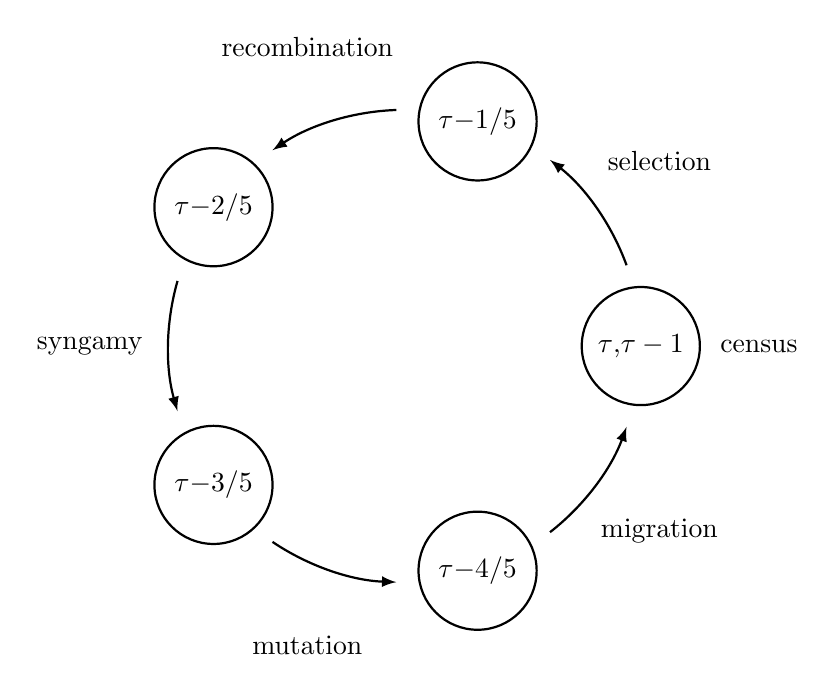
\begin{tikzpicture}
%
\def \n {5} %number of stages
\def \nm {4} %number of stages minus 1
\def \radius {3cm} %radius of lifecyle
\def \margin {20} %margin between arrows and circles
\def \names {{"selection", "recombination", "syngamy", "mutation", "migration"}} %names of stages
%
\foreach \s in {0,...,\nm}
{
  \draw[thick] ({360/\n * \s}:\radius) circle[radius=0.75cm]; %circles
  \draw[->, >=latex, thick] ({360/\n * \s + \margin}:\radius) %arrows
    arc ({360/\n * \s + \margin}:{360/\n * (\s+1) - \margin}:\radius);
  \node at  ({360/\n * (\s+0.5)}:\radius+1cm) {\pgfmathparse{\names[\s]}\pgfmathresult}; %names  
  \node at  ({360/\n * \s}:\radius) {\ifthenelse{\s=0}{$\tau$,$\tau-1$}{$\tau -$\s/\n}}; %times
}
\node at (0:\radius+1.5cm) {census};
%
\end{tikzpicture}
\caption{
Life-cycle and time notation.
}%
\label{fig:lifecycle}
\end{figure}
%
\subsection*{Migration}
%
The number of migrant alleles that arrive each generation is Poisson with mean $m$. 
Given that there are $2N'(\tau-1)p'(\tau-1)$ beneficial alleles in the next generation, the probability that any one is a new migrant is therefore $P = m/[2N'(\tau-1)p'(\tau-1)]\approx m/[2N'(\tau)p'(\tau)]$, where the approximation assumes the number of beneficial alleles changes little from one generation to the next.
The probability that at least one of $k$ beneficial alleles is a migrant is $1-(1-P)^k$, which, with rare migration, is approximately 
\begin{equation}
p_\mathrm{mig}(k,\tau) = k \frac{m}{2N'(\tau)p'(\tau)}.
\end{equation}
For a given probability of being replaced by a migrant allele, the rate of migration in a diploid model is half that of the haploid model \citep[equation 15 in][replacing $M$ with $m$]{pennings2006soft2} as there are twice as many resident alleles.
%
\subsection*{Mutation}
%
The number of beneficial alleles after mutation, $2N'(\tau-4/5)p'(\tau-4/5)$, is the number before mutation plus the number of new mutants
\begin{equation}
2N'(\tau-4/5)p'(\tau-4/5) = 2N'(\tau-3/5)p'(\tau-3/5) + u 2N'(\tau-3/5)[1-p'(\tau-3/5)].
\end{equation}
Because the population size does not change during mutation, $N'(\tau-4/5)=N'(\tau-3/5)$, the frequency of beneficial alleles after mutation is simply
\begin{equation}
p'(\tau-4/5) = p'(\tau-3/5) + u [1-p'(\tau-3/5)].
\end{equation}
The probability a beneficial allele is a new mutant is therefore $u [1-p'(\tau-3/5)]/p'(\tau-4/5)$, which, using the previous equation, is equivalent to
\begin{equation}
P = \frac{u [1-p'(\tau-4/5)]}{(1-u)p'(\tau-4/5)}.
\end{equation}
The probability that at least one of $k$ beneficial alleles is a new mutant is $1-(1-P)^k$, which, when mutation is rare, is approximately $k u [1-p'(\tau-4/5)]/p'(\tau-4/5)$.
With little change in allele frequency from one generation to the next this is
\begin{equation}
p_\mathrm{mut}(k,\tau) = k u \frac{1-p'(\tau)}{p'(\tau)}.
\end{equation}
This is equivalent to the haploid result \citep[e.g., equation 5 in][]{pennings2006soft2} as both the mutation rate and number of alleles are multiplied by the ploidy level, which cancels.
%
\subsection*{Coalescence}
%
Considering $k$ beneficial alleles at the time of census, and ignoring any migration or mutation, the probability of at least one coalescence event is then 
\begin{equation}
\binom{k}{2}\frac{1}{2N_e'(\tau-2/5)p'(\tau-2/5)},
\end{equation}
where $N_e'(\tau-2/5)$ is the effective population size at the time of syngamy.
When allele frequency and effective population size changes little from one generation to the next this is roughly
\begin{equation}
p_\mathrm{coal}(k,\tau) = \binom{k}{2}\frac{1}{2N_e'(\tau)p'(\tau)}.
\end{equation}
This is half the rate observed in a haploid model with the same population size \citep[equation 5 in][]{pennings2006soft2} as there are twice as many alleles in a diploid population.
%
\subsection*{Recombination}
%
Consider a neutral locus at recombination distance $r$ from the selected site.
Assuming weak selection such that the survivors of viability selection remain in Hardy-Weinberg proportions, the number of alleles linked to the beneficial allele after recombination is
\begin{equation}
\begin{aligned}
2 N'(\tau-2/5) p'(\tau-2/5) &= 2 N'(\tau-1/5) p'(\tau-1/5) \left[p'(\tau-1/5) + \left[1-p'(\tau-1/5) \right] (1-r) \right]\\
 &+  N'(\tau-1/5) [1-p'(\tau-1/5)] p'(\tau-1/5) r.
\end{aligned}
\end{equation}
The first term on the right hand side is the number currently linked to the beneficial allele multiplied by the probability of being in a beneficial homozygote plus the probability of being in a heterozygote but not recombining.
The second term on the right hand side is the number not currently linked with the beneficial allele times the probability of being in a heterozygote and recombining onto the beneficial background.
%
The probability an allele on the beneficial background after recombination was not there before is then
\begin{equation}
P = \frac{2 N'(\tau-1/5) [1-p'(\tau-1/5)] p'(\tau-1/5) r}{2 N'(\tau-2/5) p'(\tau-2/5)},
\end{equation}
which, because recombination does not change allele frequency or population size, is
\begin{equation}
\begin{aligned}
P &= \frac{2 N'(\tau-1/5) [1-p'(\tau-1/5)] p'(\tau-1/5) r}{2 N'(\tau-1/5) p'(\tau-1/5)}\\
&= [1-p'(\tau-1/5)] r.
\end{aligned}
\end{equation}
The probability at least one of $k$ alleles on the beneficial background recombines off is $1-(1-P)^k$, which, when recombination is rare, is approximately $k r [1-p'(\tau-1/5)]$.
Assuming allele frequency changes little through one bout of selection this is $k r [1-p'(\tau)]$.
Finally, assuming migration, mutation, and coalescence are rare, the probability that none of $k$ beneficial alleles migrates or mutates times the probability none coalesce times the probability at least one of the $k$ linked alleles recombines off is roughly \citep[table 1 in][]{hudson1988coalescent}
\begin{equation}
p_\mathrm{rec}(k,\tau) = k r [1-p'(\tau)].
\end{equation}

%%%%%%%%%%%%%%%%%%%%%%%%%%%%%%%%%%%%%%%%%%%%%%%%%
\newpage
\section*{Supplementary figures}

%%%%%%%%%%%%%%%%%%%%%%%%%%%%%%%%%%%%%%%%%%%%%%%
\begin{figure}[htb]
\centering
\begin{tikzpicture}
\node[] (A) {\includegraphics[width=0.49\linewidth]{EH_rescue_s0.2_k100_u0_m0.pdf}};
\node[right = 0 of A] (B) {\includegraphics[width=0.49\linewidth]{EH_rescue_s0.2_k1_u0_m0.pdf}};
\node[below = 0 of A] (C) {\includegraphics[width=0.49\linewidth]{EH_rescue_s0.13_k100_u0_m0.pdf}};
\node[right = 0 of C] (D) {\includegraphics[width=0.49\linewidth]{EH_rescue_s0.13_k1_u0_m0.pdf}};
\node[right = 0 of A, xshift = 0.6cm, yshift = -0.5cm, draw, rectangle, rounded corners, thick, fill=gray!50, rotate = 90] (s) {\large$\bm{s=0.20}$};
\node[right = 0 of C,  xshift = 0.6cm, yshift = -0.5cm, draw, rectangle, rounded corners, thick, fill=gray!50, rotate = 90] {\large$\bm{s=0.13}$};
\node[below = -2/3 of A, xshift = 20, draw, rectangle, rounded corners, thick, fill=gray!50] (k) {\large$\bm{\kappa=100}$};
\node[below = -2/3 of B, xshift = 20, draw, rectangle, rounded corners, thick, fill=gray!50] {\large$\bm{\kappa=1}$};
\node[right = 2cm of k, darkred, yshift = 0.25cm, draw, rectangle, rounded corners, thick, fill=darkred!25] (N) {\fontfamily{phv}\selectfont \textbf{constant $\bm{N}$}};
\node[below = 0 of N, darkblue, draw, rectangle, rounded corners, thick, fill=darkblue!25] {\fontfamily{phv}\selectfont \textbf{evol.\ rescue}};
\end{tikzpicture}
\caption{
Mean pairwise diversity, $\pi$, after a selective sweep from standing genetic variation during evolutionary rescue (blue; $d=0.05$) or in a population of roughly constant size (red; $d=0$ such that $\mathbb{E}[N(t)]=N(0)$).
The dashed curves are Equation \ref{eq:EH_rescue}.
See Figure \ref{fig:rescueSGV_heterozygosity_empirical} for additional details.
}%
\label{fig:rescueSGV_heterozygosity}
\end{figure}
%%%%%%%%%%%%%%%%%%%%%%%%%%%%%%%%%%%%%%%%%%%%%%%

%%%%%%%%%%%%%%%%%%%%%%%%%%%%%%%%%%%%%%%%%%%%%%%
\begin{figure}[htb]
\centering
\begin{tikzpicture}
\node[] (A) {\includegraphics[width=0.49\linewidth]{EH_rescue_s0.2_k0_u0.0001_m0.pdf}};
\node[right =0 of A] (B) {\includegraphics[width=0.49\linewidth]{EH_rescue_s0.2_k0_u0.00001_m0.pdf}};
\node[below =0 of A] (C) {\includegraphics[width=0.49\linewidth]{EH_rescue_s0.13_k0_u0.0001_m0.pdf}};
\node[right =0 of C] (D) {\includegraphics[width=0.49\linewidth]{EH_rescue_s0.13_k0_u0.00001_m0.pdf}};
\node[right = 0 of A, xshift = 0.6cm, yshift = -0.5cm, draw, rectangle, rounded corners, thick, fill=gray!50, rotate = 90] (s) {\large$\bm{s=0.20}$};
\node[right = 0 of C,  xshift = 0.6cm, yshift = -0.5cm, draw, rectangle, rounded corners, thick, fill=gray!50, rotate = 90] {\large$\bm{s=0.13}$};
\node[below = -2/3 of A, xshift = 20, draw, rectangle, rounded corners, thick, fill=gray!50] (k) {\large$\bm{u=10^{-4}}$};
\node[below = -2/3 of B, xshift = 20, draw, rectangle, rounded corners, thick, fill=gray!50] {\large$\bm{u=10^{-5}}$};
\node[right = 2cm of k, darkred, yshift = 0.25cm, draw, rectangle, rounded corners, thick, fill=darkred!25] (N) {\fontfamily{phv}\selectfont \textbf{constant $\bm{N}$}};
\node[below = 0 of N, darkblue, draw, rectangle, rounded corners, thick, fill=darkblue!25] {\fontfamily{phv}\selectfont \textbf{evol.\ rescue}};
\end{tikzpicture}
\caption{
Mean pairwise diversity, $\pi$, after a selective sweep from \textit{de novo} mutation during evolutionary rescue (blue; $d=0.05$) or in a population of roughly constant size (red; $d=0$).
The dashed curves are Equation \ref{eq:EH_rescue}.
See Figure \ref{fig:rescueSGV_heterozygosity_empirical} for additional details.
}%
\label{fig:rescueDNM_heterozygosity}
\end{figure}
%%%%%%%%%%%%%%%%%%%%%%%%%%%%%%%%%%%%%%%%%%%%%%%

%%%%%%%%%%%%%%%%%%%%%%%%%%%%%%%%%%%%%%%%%%%%%%%
\begin{figure}[htb]
\centering
\begin{tikzpicture}
\node[] (A) {\includegraphics[width=0.49\linewidth]{EH_rescue_s0.2_k100_u0_m0_relative.pdf}};
\node[right = 0 of A] (B) {\includegraphics[width=0.49\linewidth]{EH_rescue_s0.2_k1_u0_m0_relative.pdf}};
\node[below = 0 of A] (C) {\includegraphics[width=0.49\linewidth]{EH_rescue_s0.13_k100_u0_m0_relative.pdf}};
\node[right = 0 of C] (D) {\includegraphics[width=0.49\linewidth]{EH_rescue_s0.13_k1_u0_m0_relative.pdf}};
\node[right = 0 of A, xshift = 0.6cm, yshift = -0.5cm, draw, rectangle, rounded corners, thick, fill=gray!50, rotate = 90] (s) {\large$\bm{s=0.20}$};
\node[right = 0 of C,  xshift = 0.6cm, yshift = -0.5cm, draw, rectangle, rounded corners, thick, fill=gray!50, rotate = 90] {\large$\bm{s=0.13}$};
\node[below = -2/3 of A, xshift = 20, draw, rectangle, rounded corners, thick, fill=gray!50] (k) {\large$\bm{\kappa=100}$};
\node[below = -2/3 of B, xshift = 20, draw, rectangle, rounded corners, thick, fill=gray!50] {\large$\bm{\kappa=1}$};
\node[right = 2cm of k, darkred, yshift = 0.25cm, draw, rectangle, rounded corners, thick, fill=darkred!25] (N) {\fontfamily{phv}\selectfont \textbf{constant $\bm{N}$}};
\node[below = 0 of N, darkblue, draw, rectangle, rounded corners, thick, fill=darkblue!25] {\fontfamily{phv}\selectfont \textbf{evol.\ rescue}};
\end{tikzpicture}
\caption{
Relative mean pairwise diversity, $\pi/\overline{\pi}$, after a selective sweep from standing genetic variation during evolutionary rescue (blue; $d=0.05$) or in a population of roughly constant size (red; $d=0$ such that $\mathbb{E}[N(t)]=N(0)$).
The thick curves are $\mathbb{E}[\pi]/\mathbb{E}[\pi|\mathrm{unlinked}]$ (Equation \ref{eq:EH_rescue}).
The thinnest curves are 100 replicate simulations (rescue only for clarity) and the slightly thicker curves are simulation means (often obscured by prediction).
Parameters: $N(0)=10^4$.
}%
\label{fig:rescueSGV_heterozygosity_relative}
\end{figure}
%%%%%%%%%%%%%%%%%%%%%%%%%%%%%%%%%%%%%%%%%%%%%%%

%%%%%%%%%%%%%%%%%%%%%%%%%%%%%%%%%%%%%%%%%%%%%%%
\begin{figure}[htb]
\centering
\begin{tikzpicture}
\node[] (A) {\includegraphics[width=0.49\linewidth]{EH_rescue_s0.2_k0_u0.0001_m0_relative.pdf}};
\node[right =0 of A] (B) {\includegraphics[width=0.49\linewidth]{EH_rescue_s0.2_k0_u0.00001_m0_relative.pdf}};
\node[below =0 of A] (C) {\includegraphics[width=0.49\linewidth]{EH_rescue_s0.13_k0_u0.0001_m0_relative.pdf}};
\node[right =0 of C] (D) {\includegraphics[width=0.49\linewidth]{EH_rescue_s0.13_k0_u0.00001_m0_relative.pdf}};
\node[right = 0 of A, xshift = 0.6cm, yshift = -0.5cm, draw, rectangle, rounded corners, thick, fill=gray!50, rotate = 90] (s) {\large$\bm{s=0.20}$};
\node[right = 0 of C,  xshift = 0.6cm, yshift = -0.5cm, draw, rectangle, rounded corners, thick, fill=gray!50, rotate = 90] {\large$\bm{s=0.13}$};
\node[below = -2/3 of A, xshift = 20, draw, rectangle, rounded corners, thick, fill=gray!50] (k) {\large$\bm{u=10^{-4}}$};
\node[below = -2/3 of B, xshift = 20, draw, rectangle, rounded corners, thick, fill=gray!50] {\large$\bm{u=10^{-5}}$};
\node[right = 2cm of k, darkred, yshift = 0.25cm, draw, rectangle, rounded corners, thick, fill=darkred!25] (N) {\fontfamily{phv}\selectfont \textbf{constant $\bm{N}$}};
\node[below = 0 of N, darkblue, draw, rectangle, rounded corners, thick, fill=darkblue!25] {\fontfamily{phv}\selectfont \textbf{evol.\ rescue}};
\end{tikzpicture}
\caption{
Relative mean pairwise diversity, $\pi/\overline{\pi}$, after a selective sweep from \textit{de novo} mutation during evolutionary rescue (blue; $d=0.05$) or in a population of roughly constant size (red; $d=0$).
See Figure \ref{fig:rescueSGV_heterozygosity_relative} for details.
}%
\label{fig:rescueDNM_heterozygosity_relative}
\end{figure}
%%%%%%%%%%%%%%%%%%%%%%%%%%%%%%%%%%%%%%%%%%%%%%%


%%%%%%%%%%%%%%%%%%%%%%%%%%%%%%%%%%%%%%%%%%%%%%%
\begin{figure}[htbp]
\centering
\begin{tikzpicture}
\node[] (A1) {\includegraphics[width=0.49\linewidth]{pt_rescue_s0.2_k0_u0_m1.pdf}};
\node[below = -1cm of A1] (A2) {\includegraphics[width=0.49\linewidth]{nt_rescue_s0.2_k0_u0_m1.pdf}};
\node[right = 0cm of A1] (B1) {\includegraphics[width=0.49\linewidth]{pt_rescue_s0.2_k0_u0_m0.1.pdf}};
\node[right = 0cm of A2] (B2) {\includegraphics[width=0.49\linewidth]{nt_rescue_s0.2_k0_u0_m0.1.pdf}};
\node[below = 0cm of A2] (C1) {\includegraphics[width=0.49\linewidth]{pt_rescue_s0.13_k0_u0_m1.pdf}};
\node[below = -1cm of C1] (C2) {\includegraphics[width=0.49\linewidth]{nt_rescue_s0.13_k0_u0_m1.pdf}};
\node[right = 0cm of C1] (D1) {\includegraphics[width=0.49\linewidth]{pt_rescue_s0.13_k0_u0_m0.1.pdf}};
\node[right = 0cm of C2] (D2) {\includegraphics[width=0.49\linewidth]{nt_rescue_s0.13_k0_u0_m0.1.pdf}};
\node[right = 0.5 of A1, yshift = -2.5cm, rotate = 90, draw, rectangle, rounded corners, thick, fill=gray!50] (s) {\large$\bm{s=0.20}$};
\node[right = 0.5 of C1, yshift = -2.5cm, rotate = 90, draw, rectangle, rounded corners, thick, fill=gray!50] {\large$\bm{s=0.13}$};
\node[below = -0.6cm of A2, xshift = 20, draw, rectangle, rounded corners, thick, fill=gray!50] (k) {\large$\bm{m=1}$};
\node[below = -0.6cm of B2, xshift = 20, draw, rectangle, rounded corners, thick, fill=gray!50] {\large$\bm{m=0.1}$};
\node[right = 2cm of k, darkred, yshift = 0.25cm, draw, rectangle, rounded corners, thick, fill=darkred!25] (N) {\fontfamily{phv}\selectfont\textbf{constant $\bm{N}$}};
\node[below = 0cm of N, darkblue, draw, rectangle, rounded corners, thick, fill=darkblue!25] {\fontfamily{phv}\selectfont\textbf{evol.\ rescue}};
\end{tikzpicture}
\caption{
Allele frequency and population size during a selective sweep from migration in evolutionary rescue (blue; $d=0.05$) or in a population of roughly constant size (red; $d=0$).
See Figure \ref{fig:rescueSGV_dynamics} for details.
}%
\label{fig:rescueMIG_dynamics}
\end{figure}
%%%%%%%%%%%%%%%%%%%%%%%%%%%%%%%%%%%%%%%%%%%%%%%%

%%%%%%%%%%%%%%%%%%%%%%%%%%%%%%%%%%%%%%%%%%%%%%%%
\begin{figure}[htbp]
\centering
\begin{tikzpicture}
\node[] (A1) {\includegraphics[width=0.49\linewidth]{dynamics_rescue_s0.2_k0_u0_m1.pdf}};
\node[below = -1cm of A1] (A2) {\includegraphics[width=0.49\linewidth]{coalescent_rescue_s0.2_k0_u0_m1.pdf}};
\node[right = 0cm of A1] (B1) {\includegraphics[width=0.49\linewidth]{dynamics_rescue_s0.2_k0_u0_m0.1.pdf}};
\node[right = 0cm of A2] (B2) {\includegraphics[width=0.49\linewidth]{coalescent_rescue_s0.2_k0_u0_m0.1.pdf}};
\node[below = 0cm of A2] (C1) {\includegraphics[width=0.49\linewidth]{dynamics_rescue_s0.13_k0_u0_m1.pdf}};
\node[below = -1cm of C1] (C2) {\includegraphics[width=0.49\linewidth]{coalescent_rescue_s0.13_k0_u0_m1.pdf}};
\node[right = 0cm of C1] (D1) {\includegraphics[width=0.49\linewidth]{dynamics_rescue_s0.13_k0_u0_m0.1.pdf}};
\node[right = 0cm of C2] (D2) {\includegraphics[width=0.49\linewidth]{coalescent_rescue_s0.13_k0_u0_m0.1.pdf}};
\node[right = 0.5 of A1, yshift = -2.5cm, rotate = 90, draw, rectangle, rounded corners, thick, fill=gray!50] (s) {\large$\bm{s=0.20}$};
\node[right = 0.5 of C1, yshift = -2.5cm, rotate = 90, draw, rectangle, rounded corners, thick, fill=gray!50] {\large$\bm{s=0.13}$};
\node[below = -0.6cm of A2, xshift = 20, draw, rectangle, rounded corners, thick, fill=gray!50] (k) {\large$\bm{m=1}$};
\node[below = -0.6cm of B2, xshift = 20, draw, rectangle, rounded corners, thick, fill=gray!50] {\large$\bm{m=0.1}$};
\node[right = 2cm of k, darkred, yshift = 0.25cm, draw, rectangle, rounded corners, thick, fill=darkred!25] (N) {\fontfamily{phv}\selectfont\textbf{constant $\bm{N}$}};
\node[below = 0cm of N, darkblue, draw, rectangle, rounded corners, thick, fill=darkblue!25] {\fontfamily{phv}\selectfont\textbf{evol.\ rescue}};
\node (pt) at ($(A1) + (-0.5cm,-0.5cm)$) {\footnotesize\fontfamily{phv}\selectfont sweep};
\draw (pt) -- ($(pt)+(1.25,-1)$);
\node (nt) at ($(A1) + (-1cm,1cm)$) {\footnotesize\fontfamily{phv}\selectfont bottleneck};
\draw (nt) -- ($(nt)+(1.25,-1/2)$);
\node (rec) at ($(A2) + (-1cm,2cm)$) {\footnotesize\fontfamily{phv}\selectfont recombination};
\draw (rec) -- ($(rec)+(1.9,-1/2)$);
\node (mut) at ($(A2) + (-1cm,0.5cm)$) {\footnotesize\fontfamily{phv}\selectfont migration};
\draw (mut) -- ($(mut)+(1.4,-0.75)$);
\node (coal) at ($(A2) + (3cm,0.5cm)$) {\footnotesize\fontfamily{phv}\selectfont coalescence};
\draw (coal) -- ($(coal)+(-1.8,-0.8)$);
\end{tikzpicture}
\caption{
Timing of events in the history of a sample of size 2 at a linked neutral locus ($r=0.01$) during a selective sweep from migration in evolutionary rescue (blue; $d=0.05$) or in a population of roughly constant size (red; $d=0$).
See Figure \ref{fig:rescueSGV_timing} for details.
}%
\label{fig:rescueMIG_timing}
\end{figure}
%%%%%%%%%%%%%%%%%%%%%%%%%%%%%%%%%%%%%%%%%%%%%%%%

\end{document}